% to_cad_documentation.tex — Standalone LaTeX documentation for TO_CAD Pipeline
%
% Compile:  cd docs && pdflatex to_cad_documentation.tex  (run twice for TOC/refs)
% Requires: tikz-3dplot package, lmodern fonts

\documentclass[a4paper, 11pt, openany]{report}

% ---------------------------------------------------------------------------
% Geometry & Layout
% ---------------------------------------------------------------------------
\usepackage[margin=25mm, top=30mm, bottom=30mm]{geometry}
\usepackage{setspace}
\onehalfspacing
\usepackage{parskip}

% ---------------------------------------------------------------------------
% Fonts
% ---------------------------------------------------------------------------
\usepackage[T1]{fontenc}
\usepackage{lmodern}
\usepackage{microtype}

% ---------------------------------------------------------------------------
% Math
% ---------------------------------------------------------------------------
\usepackage{amsmath, amssymb, bm}

% ---------------------------------------------------------------------------
% Code Listings
% ---------------------------------------------------------------------------
\usepackage{listings}
\usepackage{xcolor}

\definecolor{codegreen}{rgb}{0,0.5,0}
\definecolor{codegray}{rgb}{0.5,0.5,0.5}
\definecolor{codepurple}{rgb}{0.58,0,0.82}
\definecolor{backcolour}{rgb}{0.97,0.97,0.97}

\lstdefinestyle{pythonstyle}{
    language=Python,
    backgroundcolor=\color{backcolour},
    basicstyle=\ttfamily\footnotesize,
    keywordstyle=\color{blue}\bfseries,
    commentstyle=\color{codegreen},
    stringstyle=\color{codepurple},
    numbers=left, numberstyle=\tiny\color{codegray},
    breaklines=true, frame=single,
    aboveskip=8pt, belowskip=8pt,
    showstringspaces=false,
    tabsize=4
}
\lstdefinestyle{bashstyle}{
    language=bash,
    backgroundcolor=\color{backcolour},
    basicstyle=\ttfamily\footnotesize,
    keywordstyle=\color{blue},
    breaklines=true, frame=single,
    aboveskip=8pt, belowskip=8pt,
    showstringspaces=false
}
\lstdefinestyle{textstyle}{
    basicstyle=\ttfamily\footnotesize,
    backgroundcolor=\color{backcolour},
    breaklines=true, frame=single,
    aboveskip=8pt, belowskip=8pt,
    showstringspaces=false
}

% ---------------------------------------------------------------------------
% Tables
% ---------------------------------------------------------------------------
\usepackage{booktabs}
\usepackage{longtable}
\usepackage{tabularx}
\usepackage{array}

% ---------------------------------------------------------------------------
% Figures
% ---------------------------------------------------------------------------
\usepackage{graphicx}
\usepackage{tikz}
\usepackage{tikz-3dplot}
\usetikzlibrary{arrows.meta, calc, positioning, shapes.geometric, fit}
\usepackage[subpreambles=true]{standalone}

% ---------------------------------------------------------------------------
% Cross-references & Links
% ---------------------------------------------------------------------------
\usepackage[hidelinks, bookmarksnumbered, pdfusetitle]{hyperref}
\usepackage[capitalise, noabbrev]{cleveref}

% ---------------------------------------------------------------------------
% Misc
% ---------------------------------------------------------------------------
\usepackage{enumitem}
\usepackage{caption}
\usepackage{float}
\usepackage[nottoc]{tocbibind}
\usepackage{changepage}

% ---------------------------------------------------------------------------
% Custom API function environment
% ---------------------------------------------------------------------------
\newcommand{\apifunc}[2]{%
    \paragraph{\texttt{#2}}\hfill\textit{\small #1}\par\nopagebreak
}

% ===========================================================================
%  DOCUMENT
% ===========================================================================
\begin{document}

% ---------------------------------------------------------------------------
% Title Page
% ---------------------------------------------------------------------------
\begin{titlepage}
\centering
\vspace*{4cm}
{\Huge\bfseries TO\_CAD Pipeline Documentation\par}
\vspace{1cm}
{\Large Converting 3-D SIMP Density Fields to\\Parametric CAD Models\par}
\vspace{2cm}
{\large James Jacouris\par}
\vspace{1cm}
{\large Version 1.0\par}
\vspace{0.5cm}
{\large \today\par}
\vfill
\end{titlepage}

% ---------------------------------------------------------------------------
% Front Matter
% ---------------------------------------------------------------------------
\tableofcontents
\listoffigures
\listoftables

% ===================================================================
%  CHAPTER 1: Introduction
% ===================================================================
\chapter{Introduction}
\label{ch:introduction}

\textbf{TO\_CAD} converts three-dimensional SIMP density fields into editable
parametric CAD models (beams, plates, and fused solid bodies) ready for
FreeCAD.  The pipeline chains four stages:

\begin{table}[htbp]
\caption{Pipeline stages.}
\label{tab:pipeline-stages}
\centering
\begin{tabularx}{\textwidth}{clX}
\toprule
Stage & Script / Module & What it does \\
\midrule
0 & \texttt{run\_top3d.py} & 3-D topology optimisation (Python Top3D) $\to$ density \texttt{.npz} \\
1 & \texttt{reconstruct} & Yin medial-axis thinning $\to$ beam graph + plate regions $\to$ \texttt{.json} \\
2 & \texttt{size\_opt} & Optimality-Criteria cross-section sizing \\
3 & \texttt{layout\_opt} & L-BFGS-B node-position layout optimisation \\
\bottomrule
\end{tabularx}
\end{table}

The final JSON is imported into FreeCAD via \texttt{freecad\_reconstruct.py}.

Additional capabilities include curved B\'ezier beams (\texttt{-{}-curved}),
external mesh input from STL/OBJ files (\texttt{-{}-mesh\_input}), mirror-half
symmetry enforcement (\texttt{-{}-symmetry}), and a fused solid body for STEP
export.


% ===================================================================
%  CHAPTER 2: Getting Started
% ===================================================================
\chapter{Getting Started}
\label{ch:getting-started}

% -------------------------------------------------------------------
\section{Installation}
\label{sec:installation}

\subsection{Python Dependencies}

Python 3.9 or later is required.  Create a virtual environment and install
dependencies:

\begin{lstlisting}[style=bashstyle]
python -m venv .venv
source .venv/bin/activate

# Core
pip install numpy scipy numba matplotlib

# Visualisation (optional)
pip install open3d

# Parameter tuning (optional)
pip install optuna

# Documentation (optional)
pip install sphinx sphinx-rtd-theme
\end{lstlisting}

\subsection{Verifying the Installation}

\begin{lstlisting}[style=bashstyle]
python -c "
from src.optimization.top3d import Top3D
from src.pipelines.baseline_yin.reconstruct import reconstruct_npz
from src.optimization.size_opt import optimize_size
from src.optimization.layout_opt import optimize_layout
from src.problems import load_problem_config
print('All imports OK')
"
\end{lstlisting}

\subsection{FreeCAD Macro Setup}

Copy \texttt{src/export/freecad\_reconstruct.py} to
\texttt{\textasciitilde/.FreeCAD/Macro/} and run from the FreeCAD GUI via
\textbf{Macro $\to$ Macros\ldots}.


% -------------------------------------------------------------------
\section{Quick Start}
\label{sec:quickstart}

A four-command workflow demonstrates the full pipeline.

\textbf{Step 1 --- Topology Optimisation}

\begin{lstlisting}[style=bashstyle]
python run_top3d.py \
    --nelx 60 --nely 20 --nelz 4 \
    --volfrac 0.3 --penal 3.0 --rmin 1.5 \
    --problem cantilever \
    --output output/hybrid_v2/cantilever_top3d.npz
\end{lstlisting}

\textbf{Step 2 --- Skeleton Reconstruction + Optimisation}

\begin{lstlisting}[style=bashstyle]
python run_pipeline.py \
    --skip_top3d \
    --top3d_npz output/hybrid_v2/cantilever_top3d.npz \
    --opt_loops 2 \
    --output cantilever.json
\end{lstlisting}

\textbf{Step 3 --- Interactive Preview (optional)}

\begin{lstlisting}[style=bashstyle]
python run_pipeline.py \
    --skip_top3d \
    --top3d_npz output/hybrid_v2/cantilever_top3d.npz \
    --visualize --output debug.json
\end{lstlisting}

\textbf{Step 4 --- FreeCAD Import}

Open FreeCAD, run the macro, and select the
\texttt{cantilever\_history.json} file.

\subsection{Typical Output Files}

\begin{itemize}[nosep]
    \item \texttt{*\_top3d.npz} --- density field from Stage~0
    \item \texttt{*\_1\_reconstructed.json} --- Stage~1 skeleton
    \item \texttt{*\_3\_sized\_loop1.json} --- after size optimisation
    \item \texttt{*\_2\_layout\_loop1.json} --- after layout optimisation
    \item \texttt{*.json} --- final output
    \item \texttt{*\_history.json} --- full history for FreeCAD timeline
\end{itemize}

\textbf{Tip}: For a one-shot run (Stages 0--3 combined):
\begin{lstlisting}[style=bashstyle]
python run_pipeline.py --nelx 60 --nely 20 --nelz 4 \
    --volfrac 0.3 --opt_loops 2 --output cantilever.json
\end{lstlisting}


% -------------------------------------------------------------------
\section{Pipeline Walkthrough}
\label{sec:pipeline-walkthrough}

\subsection{Stage 0 --- Topology Optimisation (Top3D)}
\label{sec:stage0}

\textbf{Entry point}: \texttt{run\_top3d.py} (called as subprocess from
\texttt{run\_pipeline.py} when \texttt{-{}-skip\_top3d} is \emph{not} given).

\textbf{Algorithm}: Pure-Python port of Sigmund's 88-line MATLAB
\texttt{top3d} code (\texttt{src.optimization.top3d}).  Uses a SIMP material
model with OC density updates and a mesh-independence filter.

\textbf{Boundary conditions}: Set via \texttt{-{}-problem}:
\begin{itemize}[nosep]
    \item \texttt{cantilever} --- fixed at $x = 0$, point load at $x = n_x$
    \item \texttt{roof} --- four corner supports, central downward load
    \item \texttt{bridge} --- bottom surface fixed, distributed top load
    \item \texttt{tagged} (pipeline default) --- BC tags propagated from
          \texttt{run\_top3d.py} into the \texttt{bc\_tags} array stored in the NPZ
\end{itemize}

\textbf{Key outputs} (stored in \texttt{.npz}):

\begin{lstlisting}[style=pythonstyle]
npz['rho']     # shape (nely, nelx, nelz), float64, density in [0, 1]
npz['bc_tags'] # shape (nely, nelx, nelz), int32; 1=fixed, 2=loaded, 3=passive
\end{lstlisting}


\subsection{Stage 1 --- Skeleton Reconstruction}
\label{sec:stage1}

\textbf{Entry point}: \texttt{reconstruct\_npz()} in
\texttt{src.pipelines.baseline\_yin.reconstruct}.

\textbf{Sub-steps}:
\begin{enumerate}[nosep]
    \item \textbf{Threshold} --- \texttt{solid = rho > vol\_thresh} creates a
          binary voxel mask.
    \item \textbf{EDT} --- \texttt{scipy.ndimage.distance\_transform\_edt(solid)}
          pre-computes the Euclidean distance transform.
    \item \textbf{Thinning} --- \texttt{thin\_grid\_yin()} iteratively removes
          simple points until a medial axis remains.  Mode selects topology:
          \texttt{mode=0} (curve-preserving), \texttt{mode=3} (hybrid).
    \item \textbf{Graph extraction} --- classifies skeleton voxels into endpoints
          ($\le 1$ neighbour), body (exactly~2), and junctions ($\ge 3$), then traces
          edges between non-body voxels.
    \item \textbf{Laplacian smoothing} --- three iterations of Laplacian averaging
          on edge waypoints to remove staircase artefacts.
    \item \textbf{Post-processing} --- collapse short edges, prune branch tips,
          RDP simplification, compute per-edge radii.
    \item \textbf{Initial radius} --- uniform radius:
          $r_0 = \sqrt{V_{\text{solid}} / (\pi \sum_i L_i)}$.
    \item \textbf{[Hybrid only]} --- two-signal zone classification, plate
          extraction, beam-plate joint creation.
    \item \textbf{Export} --- writes the graph + plate data to \texttt{.json}.
\end{enumerate}

\begin{table}[htbp]
\caption{Key Stage~1 parameters.}
\label{tab:stage1-params}
\centering
\begin{tabularx}{\textwidth}{llX}
\toprule
Parameter & Default & Effect \\
\midrule
\texttt{-{}-vol\_thresh} & 0.3 & Density threshold; lower $\to$ more voxels survive \\
\texttt{-{}-prune\_len} & 2.0\,mm & Remove branch tips shorter than this \\
\texttt{-{}-collapse\_thresh} & 2.0\,mm & Merge nodes connected by edges shorter than this \\
\texttt{-{}-rdp} & 1.0\,mm & Ramer--Douglas--Peucker epsilon for polyline simplification \\
\texttt{-{}-radius\_mode} & \texttt{uniform} & \texttt{uniform} = volume-matching; \texttt{edt} = geometric from EDT \\
\bottomrule
\end{tabularx}
\end{table}


\subsection{Stage 2 --- Size Optimisation}
\label{sec:stage2}

\textbf{Entry point}: \texttt{optimize\_size()} in \texttt{src.optimization.size\_opt}.

Uses the Optimality Criteria (OC) method to resize beam cross-section radii so
that the total frame volume matches \texttt{target\_volume} while minimising
compliance (maximising stiffness).  Iterates until the relative change in radii
is below $10^{-3}$ or \texttt{-{}-iters} is reached.


\subsection{Stage 3 --- Layout Optimisation}
\label{sec:stage3}

\textbf{Entry point}: \texttt{optimize\_layout()} in
\texttt{src.optimization.layout\_opt}.

Uses \texttt{scipy.optimize.minimize} with L-BFGS-B to move node positions
along compliance gradients, subject to:
\begin{itemize}[nosep]
    \item A move limit (\texttt{-{}-limit}, default 5\,mm per iteration)
    \item Design-domain box constraints
    \item Node snapping (\texttt{-{}-snap}) to merge nodes that drift within tolerance
\end{itemize}

Stages~2 and~3 are interleaved for \texttt{-{}-opt\_loops} iterations.  Each loop
runs \emph{Size first, then Layout}.


\subsection{Hybrid Beam+Plate Mode}
\label{sec:hybrid}

Enabled with \texttt{-{}-hybrid}.

After thinning (\texttt{mode=3}), the skeleton is classified into beam and plate
zones using a two-signal approach:

\begin{itemize}[nosep]
    \item \textbf{Signal~A} --- skeleton set-difference: voxels present in the
          \texttt{mode=3} skeleton but absent from a \texttt{mode=0} skeleton are
          plate candidates.
    \item \textbf{Signal~B} --- octant plane pattern count $\ge 4$ with $\ge 3$
          foreground neighbours identifies surface-like voxels directly.
\end{itemize}

Combined candidates are filtered by connected-component size and global
linearity to reject noise.  Final classification:
\begin{itemize}[nosep]
    \item \textbf{Plate voxels} (\texttt{zone == 1}): surface-like topology
    \item \textbf{Beam voxels} (\texttt{zone == 2}): curve-like topology
\end{itemize}

Plate regions are expanded back to full thickness via morphological dilation,
smoothed with Taubin's $\lambda/\mu$ filter, and assigned EDT-based thickness
($2 \times \text{EDT} \times \text{pitch}$).  Beam endpoints near a plate
boundary are snapped to a shared node by KD-tree lookup.


\subsection{Curved Beam Mode}

\texttt{-{}-curved} fits cubic B\'ezier curves through skeleton waypoints.
When enabled, the FEM assembler can use IGA Timoshenko curved-beam elements
(cubic Bernstein basis, 24-DOF, statically condensed to 12-DOF) for beams with
significant curvature, while short or straight beams continue to use standard
Euler--Bernoulli elements.  After each optimisation stage, control points are
re-fitted from updated node positions.


\subsection{External Mesh Input}

\texttt{-{}-mesh\_input <path>} allows the pipeline to accept an external STL
or OBJ mesh instead of running Top3D.  The mesh is voxelised at the pitch
specified by \texttt{-{}-mesh\_pitch} using trimesh.


\subsection{Symmetry Enforcement}

\texttt{-{}-symmetry x|y|z} enforces mirror symmetry about the specified axis.
The skeleton is split at the symmetry plane, one half is retained for
optimisation, and the result is reflected back.  Nodes on the symmetry plane are
fixed in the normal direction during layout optimisation.


% -------------------------------------------------------------------
\section{FreeCAD Export}
\label{sec:freecad-export}

The FreeCAD macro (\texttt{src.export.freecad\_reconstruct}) reads the pipeline
\texttt{.json} output and creates 3-D CAD geometry inside a FreeCAD document.

\subsection{Geometry Created}

\begin{itemize}[nosep]
    \item \textbf{Beams} --- swept circular tubes with hemispherical end caps,
          coloured with a radius heatmap (blue $\to$ red).
    \item \textbf{Curved beams} --- \texttt{Part.BezierCurve} piped through the
          cross-section circle.
    \item \textbf{Plates} --- polygon faces or B-spline surfaces; curved plates
          use offset mid-surfaces along vertex normals.
    \item \textbf{Fused body} --- a single solid created by batched
          \texttt{multiFuse} and \texttt{removeSplitter()}, suitable for STEP export.
    \item \textbf{History timeline} --- one FreeCAD group per pipeline stage for
          before/after comparison.
    \item \textbf{Density legend} --- 10 coloured reference cubes (red $\to$
          green) for the initial-voxels stage.
\end{itemize}

\subsection{Running the Macro}

\begin{enumerate}[nosep]
    \item Open FreeCAD (0.21+).
    \item \textbf{Macro $\to$ Macros\ldots} $\to$ Browse to
          \texttt{freecad\_reconstruct.py} $\to$ \textbf{Execute}.
    \item Select the \texttt{<name>\_history.json} file in the file picker.
    \item Wait for geometry creation (30--60\,s for large models).
\end{enumerate}

\subsection{Supported JSON Fields}

\begin{table}[htbp]
\caption{JSON fields consumed by the FreeCAD macro.}
\label{tab:freecad-json}
\centering
\begin{tabularx}{\textwidth}{lX}
\toprule
Field & Description \\
\midrule
\texttt{metadata.pitch} & Voxel size in mm; sets the global scale \\
\texttt{graph.nodes} & Node positions \texttt{[[x, y, z], \ldots]} \\
\texttt{graph.edges} & Edge list \texttt{[[u, v, r], \ldots]} \\
\texttt{curves} & Per-edge visualisation data (straight or B\'ezier) \\
\texttt{plates} & Plate geometry (vertices, connectivity, optional B-spline) \\
\texttt{history} & Voxel snapshots at each processing stage \\
\texttt{stages} & Graph states at each optimisation loop \\
\bottomrule
\end{tabularx}
\end{table}

\subsection{Known Limitations}

\begin{itemize}[nosep]
    \item Mid-surface plate geometry requires Open3D, which is not available
          inside the FreeCAD Python interpreter.
    \item Fused body Boolean operations can be slow for $> 2000$ beams.
    \item Very large models ($> 5000$ beams) may exceed FreeCAD's undo buffer.
\end{itemize}


% ===================================================================
%  CHAPTER 3: Architecture
% ===================================================================
\chapter{Architecture}
\label{ch:architecture}

% -------------------------------------------------------------------
\section{Architecture Overview}
\label{sec:arch-overview}

\subsection{Repository Layout}

\begin{lstlisting}[style=textstyle]
TO_CAD/
+-- run_pipeline.py            # Main orchestrator (CLI + Python API)
+-- run_top3d.py               # Stage 0: topology optimisation
+-- run_top3d_rocker_arm.py    # Rocker-arm specific Top3D script
+-- tune_parameters.py         # Optuna parameter search
|
+-- src/
|   +-- optimization/
|   |   +-- top3d.py           # Python Top3D solver (SIMP + OC)
|   |   +-- fem.py             # 3-D frame FEA (straight + curved)
|   |   +-- size_opt.py        # OC radius sizing
|   |   +-- layout_opt.py      # L-BFGS-B node-position optimisation
|   |   +-- symmetry.py        # Mirror-half symmetry enforcement
|   |
|   +-- pipelines/
|   |   +-- baseline_yin/
|   |       +-- reconstruct.py      # Stage 1 orchestrator + JSON export
|   |       +-- thinning.py         # Yin medial-axis thinning
|   |       +-- topology.py         # Topological predicates (Numba)
|   |       +-- graph.py            # Skeleton -> graph extraction
|   |       +-- postprocessing.py   # Graph pruning / cleanup
|   |       +-- plate_extraction.py # Plate region recovery (hybrid)
|   |       +-- joint_creation.py   # Beam-plate joint snapping
|   |       +-- surface_fitting.py  # B-spline plate mid-surfaces
|   |       +-- visualization.py    # Open3D / Matplotlib visualisation
|   |
|   +-- mesh_import/
|   |   +-- mesh_voxelizer.py  # External STL/OBJ -> voxel grid
|   |
|   +-- problems/
|   |   +-- __init__.py        # load_problem_config() factory
|   |   +-- cantilever.py
|   |   +-- tagged_problem.py  # Tag-based BC propagation
|   |   +-- generic.py
|   |
|   +-- curves/
|   |   +-- spline.py          # Cubic Bezier fitting & sanitisation
|   |
|   +-- export/
|   |   +-- freecad_reconstruct.py  # FreeCAD macro
|   |
|   +-- tuning/
|       +-- pipeline_runner.py  # Subprocess wrapper for trials
|       +-- metrics.py          # Geometry fidelity metrics
|
+-- docs/                       # Documentation
\end{lstlisting}


\subsection{Module Dependency Graph}

\begin{figure}[htbp]
\centering
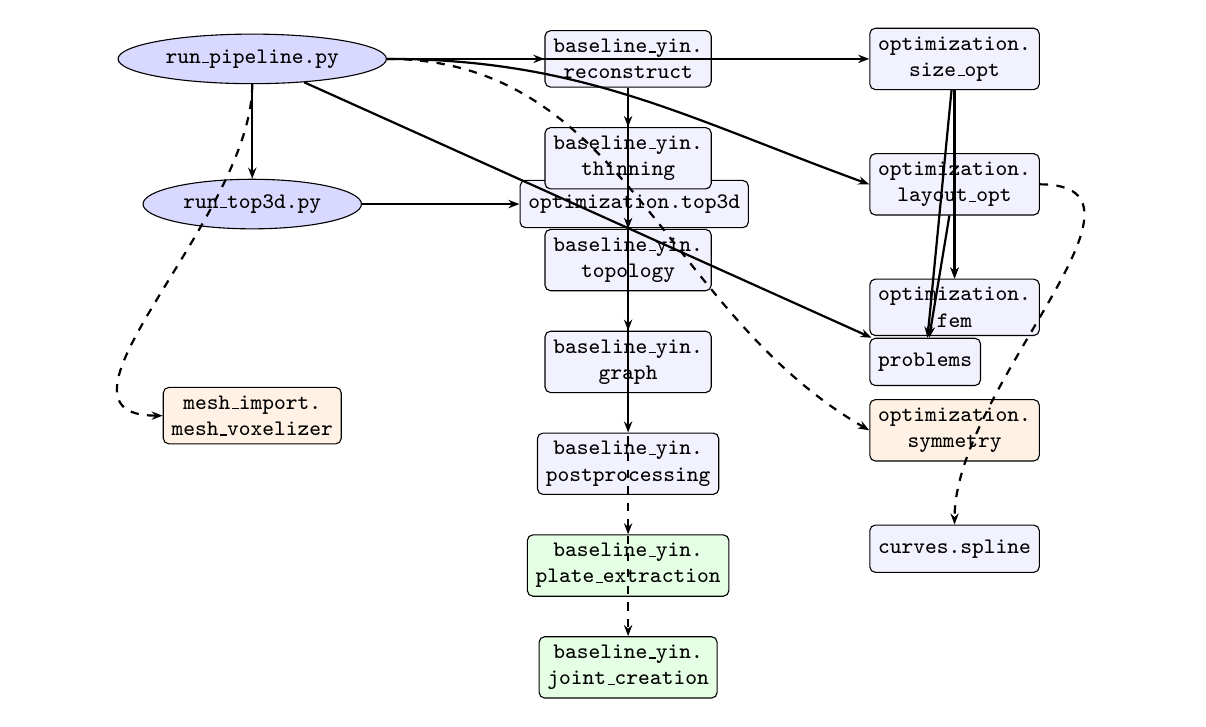
\begin{tikzpicture}[
    node distance=8mm and 14mm,
    every node/.style={
        draw, rounded corners=2pt, font=\footnotesize\ttfamily,
        fill=blue!5, minimum height=6mm, inner sep=3pt, align=center
    },
    orch/.style={ellipse, fill=blue!15},
    hybrid/.style={fill=green!10},
    optional/.style={fill=orange!10},
    edge/.style={-{Stealth[length=4pt]}, thick},
    dashedge/.style={-{Stealth[length=4pt]}, thick, dashed},
]
% Column 1: Orchestrators
\node[orch] (runpipe) {run\_pipeline.py};
\node[orch, below=12mm of runpipe] (runtop) {run\_top3d.py};

% Column 2: Stage 0
\node[right=20mm of runtop] (top3d) {optimization.top3d};

% Column 3: Stage 1
\node[right=20mm of runpipe] (recon) {baseline\_yin.\\reconstruct};
\node[below=5mm of recon] (thin) {baseline\_yin.\\thinning};
\node[below=5mm of thin] (topo) {baseline\_yin.\\topology};
\node[below=5mm of topo] (graphm) {baseline\_yin.\\graph};
\node[below=5mm of graphm] (postproc) {baseline\_yin.\\postprocessing};
\node[hybrid, below=5mm of postproc] (plateext) {baseline\_yin.\\plate\_extraction};
\node[hybrid, below=5mm of plateext] (jointcr) {baseline\_yin.\\joint\_creation};

% Column 4: Stages 2-3
\node[right=20mm of recon] (sizeopt) {optimization.\\size\_opt};
\node[below=8mm of sizeopt] (layoutopt) {optimization.\\layout\_opt};
\node[below=8mm of layoutopt] (fem) {optimization.\\fem};

% Support modules
\node[optional, below=8mm of fem] (symm) {optimization.\\symmetry};
\node[right=20mm of graphm] (problems) {problems};
\node[optional, below=20mm of runtop] (meshvox) {mesh\_import.\\mesh\_voxelizer};
\node[below=8mm of symm] (spline) {curves.spline};

% Edges
\draw[edge] (runpipe) -- (runtop);
\draw[edge] (runtop) -- (top3d);
\draw[edge] (runpipe) -- (recon);
\draw[edge] (recon) -- (thin);
\draw[edge] (thin) -- (topo);
\draw[edge] (recon) -- (graphm);
\draw[edge] (recon) -- (postproc);
\draw[dashedge] (recon) -- (plateext);
\draw[dashedge] (recon) -- (jointcr);
\draw[edge] (runpipe) -- (sizeopt);
\draw[edge] (runpipe.east) to[out=0,in=160] (layoutopt.west);
\draw[edge] (sizeopt) -- (fem);
\draw[edge] (layoutopt) -- (fem);
\draw[edge] (sizeopt) -- (problems);
\draw[edge] (layoutopt) -- (problems);
\draw[edge] (runpipe) -- (problems);
\draw[dashedge] (runpipe.south) to[out=-90,in=180] (meshvox.west);
\draw[dashedge] (layoutopt.east) to[out=0,in=90] (spline.north);
\draw[dashedge] (runpipe.east) to[out=0,in=150] (symm.west);
\end{tikzpicture}
\caption{Pipeline module dependencies.  Dashed edges indicate hybrid-only or optional paths.
Green-filled modules are hybrid-only; orange-filled are optional.}
\label{fig:module-deps}
\end{figure}


\subsection{Design Decisions}

\begin{description}[style=nextline]
    \item[Classify after thinning (hybrid mode)]
    Zone classification is applied \emph{after} a single hybrid thinning pass
    (\texttt{mode=3}), not to the original solid.  A two-signal approach
    combines skeleton set-difference with octant plane pattern counting.

    \item[Separate JSON edge format \texttt{[u, v, r]}]
    All JSON edge lists use exactly three elements: node index \texttt{u}, node
    index \texttt{v}, radius \texttt{r} (mm).

    \item[Direct Python API for Stage~1]
    \texttt{reconstruct\_npz()} is a clean Python-callable API.
    \texttt{run\_pipeline.py} calls it directly (no subprocess).

    \item[Dual FEM element library]
    The default uses 12-DOF straight Euler--Bernoulli beam elements.
    When \texttt{-{}-curved} is specified, an IGA Timoshenko element is
    available; interior DOFs are statically condensed to a 12-DOF interface.

    \item[Shared beam--plate volume budget]
    In hybrid mode, beam radii and plate thicknesses are co-optimised under a
    single volume constraint via the OC update.

    \item[Symmetry by mirror-half skeleton]
    When \texttt{-{}-symmetry} is given, the skeleton is split at the symmetry
    plane, one half is optimised, and the result is reflected back.
\end{description}


% -------------------------------------------------------------------
\section{Data Flow}
\label{sec:data-flow}

\subsection{Stage 0 \texorpdfstring{$\to$}{to} Stage 1: NPZ Format}

\texttt{run\_top3d.py} writes a NumPy \texttt{.npz} archive:

\begin{lstlisting}[style=pythonstyle]
np.savez(output_path,
    rho=rho,        # shape (nely, nelx, nelz), float64 in [0, 1]
    bc_tags=bc_tags  # shape (nely, nelx, nelz), int32; 1=fixed, 2=loaded
)
\end{lstlisting}

\textbf{Index order}: Top3D uses \texttt{(nely, nelx, nelz)} (row-major MATLAB
convention).  When converting to world coordinates, indices are reordered to
\texttt{[nelx, nely, nelz]} by taking \texttt{indices[:, [1, 0, 2]]}.


\subsection{Stage 1 Output: JSON Schema}

Key top-level keys (see \cref{sec:json-schema} for the full reference):

\begin{lstlisting}[style=textstyle]
{
  "metadata": { "pitch": 1.0, "units": "mm", "vol_thresh": 0.3, ... },
  "graph":    { "nodes": [...], "edges": [...], "node_tags": {...} },
  "curves":   [...],
  "plates":   [...],
  "joints":   [...],
  "history":  [...]
}
\end{lstlisting}


\subsection{Stages 2 \texorpdfstring{\&}{and} 3: In-Memory Arrays}

Size and layout optimisation operate on NumPy arrays extracted from the JSON:

\begin{lstlisting}[style=pythonstyle]
nodes = np.array(data['graph']['nodes'])   # (N, 3) float64, mm
edges = np.array([[e[0], e[1]] for e in data['graph']['edges']], dtype=int)
radii = np.array([e[2] for e in data['graph']['edges']])  # (M,) mm
\end{lstlisting}


\subsection{Pipeline History Object}

\texttt{run\_pipeline.py} assembles a history object for FreeCAD containing
per-voxel snapshots (type \texttt{"voxels"}) and per-graph snapshots (type
\texttt{"graph"}).  The \texttt{stages} list contains the full geometry at each
optimisation stage for the FreeCAD timeline feature.


\subsection{External Mesh Input: NPZ Format}

When \texttt{-{}-mesh\_input} is given, the NPZ contains only \texttt{rho}
(binary, float32); no \texttt{bc\_tags} are generated.

\begin{lstlisting}[style=pythonstyle]
np.savez(output_path,
    rho=rho  # shape (nely, nelx, nelz), float32, binary {0.0, 1.0}
)
\end{lstlisting}


\subsection{Symmetry Data Flow}

When \texttt{-{}-symmetry} is specified:
\begin{enumerate}[nosep]
    \item Edges crossing the symmetry plane are split at the plane intersection.
    \item One half of the skeleton is retained.
    \item After optimisation, the result is reflected and merged back.
    \item Nodes on the symmetry plane are constrained in the plane-normal
          direction during layout optimisation.
\end{enumerate}


\subsection{BC Tag Propagation}

BC tags flow from Top3D through the entire pipeline:
\begin{enumerate}[nosep]
    \item \texttt{run\_top3d.py} sets \texttt{bc\_tags[voxel] = 1} (fixed) or
          \texttt{2} (loaded).
    \item \texttt{thin\_grid\_yin()} preserves tagged voxels from deletion.
    \item \texttt{extract\_graph()} assigns \texttt{node\_tags} by majority vote
          of voxel tags at each node cluster.
    \item \texttt{TaggedProblem} reads \texttt{node\_tags} from the JSON and
          applies fixed DOFs / loads accordingly.
\end{enumerate}


% -------------------------------------------------------------------
\section{Algorithms}
\label{sec:algorithms}

\subsection{Top3D --- Topology Optimisation (Stage 0)}
\label{sec:alg-top3d}

\texttt{src.optimization.top3d} implements the 3-D extension of Sigmund's
88-line MATLAB \texttt{top} code, extended with BC tag generation, a
conjugate-gradient solver, and convergence history tracking.

\textbf{Material model}: SIMP (Solid Isotropic Material with Penalisation)

\begin{equation}
\label{eq:simp}
E(\rho_e) = E_{\min} + \rho_e^p (E_0 - E_{\min})
\end{equation}

where $p$ is the penalisation exponent (\texttt{-{}-penal}, default~3),
$E_0$ is the solid modulus, and $E_{\min} = 10^{-9}$.

\textbf{Objective}: Minimise compliance $C = \mathbf{F}^\top \mathbf{u}$
subject to a volume fraction limit $V_f$:

\begin{equation}
\label{eq:top3d-obj}
\min_{\boldsymbol{\rho}} \; C = \mathbf{F}^\top \mathbf{u}
\quad \text{s.t.} \quad
\mathbf{K}\mathbf{u} = \mathbf{F}, \quad
\frac{1}{V_0}\sum_e \rho_e v_e \le V_f, \quad
0 \le \rho_e \le 1
\end{equation}

\textbf{Sensitivity}:

\begin{equation}
\label{eq:sensitivity}
\frac{\partial C}{\partial \rho_e}
= -p\,(E_0 - E_{\min})\,\rho_e^{p-1}\,
  \mathbf{u}_e^\top \mathbf{K}_E \mathbf{u}_e
\end{equation}

where $\mathbf{K}_E$ is the unit-modulus element stiffness matrix.
Sensitivities are averaged over each element's neighbourhood within radius
$r_{\min}$ to suppress checkerboard patterns.

\textbf{Density update}: Optimality Criteria

\begin{equation}
\label{eq:oc-update}
\rho_e^{\,\text{new}} = \rho_e \cdot B_e^{\eta}
\end{equation}

where $B_e = -\partial C/\partial \rho_e / (\lambda\,\partial V/\partial \rho_e)$
and $\lambda$ is found by bisection to satisfy the volume constraint.
Iteration continues until $\max_e |\Delta\rho_e| < 0.01$.

\textbf{Mesh-independence filter}: Weighted average over a ball of radius
\texttt{-{}-rmin}

\begin{equation}
\label{eq:filter}
\hat{\rho}_e = \frac{\sum_{f} H_{ef} \rho_f}{\sum_f H_{ef}}, \quad
H_{ef} = \max(0, r_{\min} - \Delta(e,f))
\end{equation}

\textbf{Element}: 8-node hexahedral H8 with trilinear shape functions.
Stiffness matrix pre-computed by \texttt{lk\_H8()} and assembled via
vectorised indexing.  Sparse system solved with
\texttt{scipy.sparse.linalg.spsolve}.

\textbf{Binarisation}: The converged density field is binarised before Stage~1:

\begin{equation}
\label{eq:binarise}
\text{solid}_e =
\begin{cases}
1 & \rho_e > v_t \\
0 & \text{otherwise}
\end{cases}
\end{equation}

where $v_t = 0.30$ (\texttt{-{}-vol\_thresh}).  BC-tagged voxels are retained
regardless of density.

\subsubsection{Boundary-Condition Tag Generation}

Before optimisation, each element is assigned an integer tag encoding its
structural role:

\begin{itemize}[nosep]
    \item \texttt{tag = 1} \textbf{(support)}: shares a node with a
          fixed-displacement DOF.
    \item \texttt{tag = 2} \textbf{(load)}: shares a node with an applied force.
    \item \texttt{tag = 3} \textbf{(passive)}: excluded from the design domain.
\end{itemize}

Tags~1 and~2 propagate through Stages~1--3, serving two roles:
(1)~thinning protection --- tagged voxels are never deleted during
skeletonisation; and (2)~frame boundary conditions --- tagged nodes supply
fixed DOFs and loads to the frame solver.


\subsection{Skeletonisation (Stage 1)}
\label{sec:alg-skeleton}

\subsubsection{Yin Medial-Axis Thinning}

\texttt{src.pipelines.baseline\_yin.thinning} implements the 3-D parallel
directional thinning algorithm by Yin (2002).

\textbf{Core idea}: Iteratively peel voxels from the surface of the binary
solid, one layer at a time, until only a one-voxel-wide skeleton remains.

\textbf{Simple point test}: A voxel is only removed if its deletion does not
disconnect any material or merge any void regions.  The test examines the
voxel's $3 \times 3 \times 3$ neighbourhood: the 26-connected material must
form a single cluster, and the 6-connected void must also form a single cluster.

\textbf{Directional sweeps}: Each iteration sweeps in 6 axis-aligned directions
($\pm X, \pm Y, \pm Z$).  Candidates are re-checked before deletion because
an earlier removal can change a later candidate's neighbourhood.

\textbf{Unconditionally excluded voxels}:
\begin{enumerate}[nosep]
    \item \textbf{BC-tagged voxels} (\texttt{tag > 0}): support and load voxels
          are preserved.
    \item \textbf{End voxels} ($\le 1$ neighbour): prevents thin chains from
          eroding entirely.
    \item \textbf{Surface points} (mode 1/3 only): voxels bounding a 2-D medial
          surface are retained.
\end{enumerate}

\textbf{Numba acceleration}: Critical loops use \texttt{@njit(parallel=True)}.

\textbf{Thinning modes}:

\begin{table}[htbp]
\caption{Thinning modes and preserved topology.}
\label{tab:thinning-modes}
\centering
\begin{tabularx}{\textwidth}{clX}
\toprule
Mode & Name & Preserved topology \\
\midrule
0 & Curve-preserving & Curve endpoints; surfaces collapsed to medial curves \\
1 & Surface-preserving & Surface voxels retained; curves collapsed \\
3 & Hybrid (surface + curve) & Both endpoints and surface voxels preserved \\
\bottomrule
\end{tabularx}
\end{table}


\subsubsection{Graph Extraction}

\texttt{extract\_graph()} converts skeleton voxels into a graph:

\begin{enumerate}[nosep]
    \item \textbf{BC tag cluster collapsing}: Connected clusters of BC-tagged
          voxels are collapsed to single centroid nodes.
    \item \textbf{Node classification}: endpoint ($\le 1$ neighbour), body
          (exactly~2), junction ($\ge 3$).
    \item \textbf{Edge tracing}: BFS through degree-2 voxels traces the skeleton
          path between nodes.
    \item \textbf{Laplacian smoothing}: Three iterations; interior waypoints
          move halfway toward midpoint of neighbours.
    \item \textbf{BC tag assignment}: each node inherits the dominant BC tag.
\end{enumerate}


\subsubsection{Graph Post-processing}

\begin{enumerate}[nosep]
    \item \textbf{Edge collapse}: Pairs connected by edges shorter than
          \texttt{-{}-collapse\_thresh} are merged.
    \item \textbf{Branch pruning}: Degree-1 leaves on edges shorter than
          \texttt{-{}-prune\_len} are removed.
    \item \textbf{Geometric simplification}: Ramer--Douglas--Peucker algorithm
          reduces waypoints within \texttt{-{}-rdp} tolerance.
\end{enumerate}


\subsubsection{Initial Radius Assignment}

Each edge receives an initial cross-sectional radius by uniform volume-matching:

\begin{equation}
\label{eq:radius-init}
r_0 = \sqrt{\frac{V_{\text{solid}}}{\pi \sum_i L_i}}
\end{equation}

where $V_{\text{solid}}$ is the total solid voxel volume and $L_i$ the smoothed
polyline length of edge~$i$.


\subsection{Two-Signal Zone Classification (Hybrid)}
\label{sec:alg-zone}

\texttt{classify\_skeleton\_post\_thinning()} partitions the skeleton into
surface and beam zones by combining two complementary topological signals.

\textbf{Signal~A} (set-difference): Voxels present in the hybrid skeleton
(\texttt{mode~3}) but absent from a curve-only skeleton (\texttt{mode~0}):

\begin{equation}
\label{eq:signal-a}
A = \mathcal{S}_3 \setminus \mathcal{S}_0
\end{equation}

\textbf{Signal~B} (octant plane patterns): A voxel is a surface candidate if
$\ge 4$ octants match known planar configurations AND the voxel has $\ge 3$
skeleton neighbours.

\textbf{Combination}: Plate candidates are the union:

\begin{equation}
\label{eq:zone-union}
\text{candidates} = A \cup B
\end{equation}

The union is segmented into 26-connected regions, filtered by minimum size and
elongation, and assigned as surface zones.  Remaining voxels become beam zones.


\subsection{Hybrid Surface Extraction and Joint Creation}

\textbf{Surface extraction}: Full-thickness regions are recovered by
morphological dilation into the original solid, constrained to avoid beam zones.
The boundary is meshed, smoothed by Taubin filtering, and annotated with
per-vertex thickness: $t_v = 2 \times \text{EDT}(v) \times \text{pitch}$.

\textbf{Joint creation}: Beam nodes near a surface boundary are snapped onto
the nearest surface vertex using a KD-tree, creating shared nodes at each
beam-to-surface interface.


\subsection{Frame FEA}
\label{sec:alg-fea}

\subsubsection{Straight Beam Element}

\texttt{solve\_frame()} assembles a 3-D Euler--Bernoulli frame stiffness matrix.

\textbf{Element}: 2-node 3-D beam with 6~DOF per node
($u_x, u_y, u_z, \theta_x, \theta_y, \theta_z$).  Local stiffness
$\mathbf{K}_e$ (12$\times$12) is computed analytically from beam length, Young's
modulus $E$, and cross-section radius $r$ (area $A = \pi r^2$, moment of inertia
$I = \pi r^4/4$).

\textbf{Assembly}:
\begin{equation}
\label{eq:assembly}
\mathbf{K} = \sum_e \mathbf{T}_e^\top \mathbf{K}_e \mathbf{T}_e
\end{equation}

where $\mathbf{T}_e$ is the 12$\times$12 rotation matrix aligning the local
beam axis to the global frame.

\textbf{Solve}: Sparse LU via \texttt{spsolve(K\_ff, f\_f)} where subscript $f$
denotes free DOFs.

\textbf{Compliance}: $C = \mathbf{F}^\top \mathbf{u}$ (scalar).

\textbf{Gradient}:
$\partial C / \partial r_e = -\mathbf{u}_e^\top (\partial \mathbf{K}_e / \partial r_e) \mathbf{u}_e$,
evaluated analytically.


\subsubsection{Curved Beam Element (IGA Timoshenko)}

When \texttt{-{}-curved} is enabled, a cubic B\'ezier curve is fitted to each
skeleton edge and a curved finite element is built on the same basis.

\textbf{B\'ezier fitting}: With endpoints $\mathbf{P}_0$ and $\mathbf{P}_3$
fixed, interior control points $\mathbf{P}_1$ and $\mathbf{P}_2$ are found by
least-squares fitting.  Two constraints prevent degenerate curves:

\begin{itemize}[nosep]
    \item \textbf{Chord monotonicity}: $0 \le t_1 \le t_2 \le L$
    \item \textbf{Perpendicular bulge limit}: lateral deviation is clamped
\end{itemize}

\textbf{Timoshenko formulation}: A Timoshenko formulation captures
axial-bending coupling from centreline curvature.  The cubic Bernstein basis
describes both geometry and displacement (isogeometric analysis).  Four control
points give 24~DOFs.

\textbf{Static condensation}: Interior DOFs are eliminated:

\begin{equation}
\label{eq:condensation}
\mathbf{K}_{\text{cond}} = \mathbf{K}_{bb}
- \mathbf{K}_{bi}\,\mathbf{K}_{ii}^{-1}\,\mathbf{K}_{ib}
\end{equation}

where $b$ and $i$ denote boundary ($\mathbf{P}_0, \mathbf{P}_3$) and interior
($\mathbf{P}_1, \mathbf{P}_2$) DOFs, making the curved element a drop-in
replacement.


\subsection{Frame Re-optimisation (Stages 2--3)}
\label{sec:alg-reopt}

\subsubsection{Optimality Criteria Sizing (Stage 2)}

\texttt{optimize\_size()} adjusts every beam radius to minimise compliance while
keeping total frame volume equal to the solid volume from Stage~1.  In hybrid
mode the constraint includes shell contributions:
$\sum_i \pi r_i^2 L_i + \sum_j A_j h_j = V_{\text{target}}$.

\begin{equation}
\label{eq:oc-size}
r_i^{\,\text{new}} = \operatorname{clip}_{[r_i(1-m),\; r_i(1+m)]}
\left( r_i \left( \frac{-\partial C / \partial r_i}
{\lambda\;\partial V / \partial r_i} \right)^{\!\eta} \right)
\end{equation}

where $m = 0.2$ limits change per iteration, $\eta = 0.5$ is a damping
exponent, and $\lambda$ enforces the volume constraint via bisection.  Both
sensitivities ($\partial C/\partial r_i$,
$\partial V/\partial r_i = 2\pi r_i L_i$) are evaluated analytically.

\textbf{Convergence}: Iteration terminates when the maximum radius change falls
below $10^{-3}$, or after 50 iterations.


\subsubsection{L-BFGS-B Layout Optimisation (Stage 3)}

\texttt{optimize\_layout()} repositions the free nodes:

\begin{equation}
\label{eq:layout}
\min_{\mathbf{x}} \; C(\mathbf{x}) \quad \text{s.t.} \;
\mathbf{x}_{\min} \le \mathbf{x} \le \mathbf{x}_{\max}
\end{equation}

Each free node may move a limited distance.  BC-tagged and loaded nodes remain
fixed.  After convergence, nodes within \texttt{snap\_dist} are merged.


\subsubsection{Alternating Convergence}

Size and layout alternate in cycles (Stage~2 then Stage~3), controlled by
\texttt{-{}-opt\_loops} (default~2).  Size runs first because uniform radii give
all members near-identical sensitivities; once a non-uniform distribution is
established, layout can meaningfully reposition nodes.


\subsection{External Mesh Input}
\label{sec:alg-mesh}

External TO results from commercial solvers can be imported as STL/OBJ meshes
via \texttt{mesh\_voxelizer}.  The mesh is voxelised at \texttt{-{}-mesh\_pitch}
using trimesh, with interior automatically filled.  EDT-based radius assignment
is used.


\subsection{Symmetry Enforcement}
\label{sec:alg-symmetry}

\texttt{src.optimization.symmetry} detects symmetric node/edge pairs by
reflecting positions across user-specified planes, then enforces symmetry via
radius averaging (size opt) and a soft penalty plus exact projection (layout
opt).


% -------------------------------------------------------------------
\section{JSON Output Schema}
\label{sec:json-schema}

Every stage of the pipeline writes or reads a \texttt{.json} file.

\subsection{Top-Level Structure}

\begin{lstlisting}[style=textstyle]
{
  "metadata": { ... },
  "graph":    { ... },
  "curves":   [ ... ],
  "plates":   [ ... ],
  "joints":   [ ... ],
  "history":  [ ... ]
}
\end{lstlisting}


\subsection{\texttt{metadata}}

\begin{table}[htbp]
\caption{Metadata fields.}
\label{tab:json-metadata}
\centering
\begin{tabularx}{\textwidth}{llX}
\toprule
Key & Type & Description \\
\midrule
\texttt{method} & str & \texttt{"Baseline Yin"} \\
\texttt{pitch} & float & Voxel size in mm \\
\texttt{units} & str & \texttt{"mm"} \\
\texttt{target\_volume} & float & Total solid volume (mm\textsuperscript{3}) from Stage~0 \\
\texttt{design\_bounds} & [[x,y,z],[x,y,z]] & Axis-aligned bounding box \\
\texttt{vol\_thresh} & float & Density threshold used to binarise \\
\texttt{plate\_mode} & str & \texttt{"bspline"}, \texttt{"voxel"}, or \texttt{"mesh"} \\
\texttt{load\_force} & [fx, fy, fz] & Applied load vector \\
\bottomrule
\end{tabularx}
\end{table}


\subsection{\texttt{graph}}

\begin{table}[htbp]
\caption{Graph fields.}
\label{tab:json-graph}
\centering
\begin{tabularx}{\textwidth}{llX}
\toprule
Key & Type & Description \\
\midrule
\texttt{nodes} & \texttt{[[x,y,z], \ldots]} & Node world positions (mm), length $N$ \\
\texttt{edges} & \texttt{[[u,v,r], \ldots]} & $u$, $v$ = 0-based node indices; $r$ = radius (mm) \\
\texttt{node\_tags} & \texttt{\{"i": tag, \ldots\}} & 1 = fixed, 2 = loaded, 0 = free \\
\bottomrule
\end{tabularx}
\end{table}


\subsection{\texttt{curves}}

One entry per edge, in the same order as \texttt{graph.edges}.

\textbf{Straight beam} (no \texttt{-{}-curved}):
\begin{lstlisting}[style=textstyle]
{ "points": [[x, y, z, r], ...] }
\end{lstlisting}

\textbf{Curved beam} (\texttt{-{}-curved}):
\begin{lstlisting}[style=textstyle]
{
  "ctrl_pts": [[x1,y1,z1], [x2,y2,z2]],
  "points":   [[x, y, z, r], ...],
  "radius":   r
}
\end{lstlisting}


\subsection{\texttt{plates}}

Each plate entry:
\begin{lstlisting}[style=textstyle]
{
  "id":                   0,
  "voxels":               [[x,y,z], ...],
  "vertices":             [[x,y,z], ...],
  "faces":                [[i,j,k], ...],
  "thickness":            [t0, t1, ...],
  "connection_node_ids":  [n0, n1, ...],
  "bspline_surface":      { "grid_u": [...], "grid_v": [...], "points": [...] }
}
\end{lstlisting}


\subsection{\texttt{joints}}

\begin{lstlisting}[style=textstyle]
{
  "plate_id":  0,
  "node_id":   3,
  "location":  [x, y, z],
  "direction": [dx, dy, dz],
  "radius":    r,
  "type":      "fillet"
}
\end{lstlisting}


\subsection{\texttt{history}}

A list of snapshots, one per processing step.  Two types:

\textbf{Voxel snapshot} (initial solid, skeleton, zone classification):
\begin{lstlisting}[style=textstyle]
{
  "type":   "voxels",
  "step":   "1_Initial_Voxels",
  "points": [[x,y,z], ...],
  "colors": [[r,g,b], ...]
}
\end{lstlisting}

\textbf{Graph snapshot} (after each postprocessing step):
\begin{lstlisting}[style=textstyle]
{
  "type":   "graph",
  "step":   "3_Raw_Graph",
  "nodes":  [[x,y,z], ...],
  "edges":  [[u, v, r, [waypoints...]], ...],
  "plates": [ ... ]
}
\end{lstlisting}


% -------------------------------------------------------------------
% Problem Setup Figures
% -------------------------------------------------------------------

\begin{figure}[htbp]
\centering
% roof_problem_setup.tex — Roof Structure Problem Setup (40 × 40 × 20)
%
% Standalone preview:  pdflatex roof_problem_setup.tex
% Dissertation usage:  % roof_problem_setup.tex — Roof Structure Problem Setup (40 × 40 × 20)
%
% Standalone preview:  pdflatex roof_problem_setup.tex
% Dissertation usage:  % roof_problem_setup.tex — Roof Structure Problem Setup (40 × 40 × 20)
%
% Standalone preview:  pdflatex roof_problem_setup.tex
% Dissertation usage:  \input{figures/roof_problem_setup}

\documentclass[tikz,border=5mm]{standalone}
\usepackage{tikz,tikz-3dplot}
\usetikzlibrary{arrows.meta, calc}
\usepackage{amsmath}

\begin{document}

\tdplotsetmaincoords{72}{130}

\begin{tikzpicture}[tdplot_main_coords, scale=0.11]

% ── Parameters ──────────────────────────────────────────────────────
\def\NX{40}  \def\NY{40}  \def\NZ{20}
\def\arrowlen{6}

% ── Colours ─────────────────────────────────────────────────────────
\definecolor{boxcol}{HTML}{2C3E50}
\definecolor{backedge}{HTML}{B0BEC5}
\definecolor{loadred}{HTML}{C0392B}
\definecolor{fixblue}{HTML}{2471A3}
\definecolor{loadfill}{HTML}{E74C3C}
\definecolor{dimcol}{HTML}{78909C}

% ====================================================================
%  LAYER 1: BACK EDGES (dashed)
% ====================================================================
\draw[backedge, dashed, line width=0.3pt]
  (0,\NY,0) -- (\NX,\NY,0) -- (\NX,\NY,\NZ)
  (0,\NY,0) -- (0,\NY,\NZ) -- (\NX,\NY,\NZ)
  (0,0,0) -- (0,\NY,0);

% ====================================================================
%  LAYER 2: SUPPORT MARKERS
% ====================================================================
\newcommand{\supportmarker}[2]{%
  \fill[fixblue, opacity=0.9]
    (#1,#2,0) -- ({#1-1.4},{#2},-2) -- ({#1+1.4},{#2},-2) -- cycle;
  \draw[fixblue!65!black, line width=0.3pt]
    (#1,#2,0) -- ({#1-1.4},{#2},-2) -- ({#1+1.4},{#2},-2) -- cycle;
  \draw[fixblue!55!black, line width=0.4pt]
    ({#1-2},{#2},-2) -- ({#1+2},{#2},-2);
  \foreach \hx in {-1.2,-0.4,0.4,1.2} {
    \draw[fixblue!30!black, line width=0.18pt]
      ({#1+\hx},{#2},-2) -- ({#1+\hx-0.5},{#2},-2.8);
  }
}
\supportmarker{1}{1}
\supportmarker{39}{1}
\supportmarker{1}{39}
\supportmarker{39}{39}

% ====================================================================
%  LAYER 3: FRONT / VISIBLE BOX EDGES
% ====================================================================
\draw[boxcol, line width=0.8pt]
  (0,0,0) -- (\NX,0,0) -- (\NX,0,\NZ) -- (0,0,\NZ) -- cycle;
\draw[boxcol, line width=0.8pt]
  (\NX,0,0) -- (\NX,\NY,0)
  (\NX,0,\NZ) -- (\NX,\NY,\NZ)
  (0,0,\NZ) -- (0,\NY,\NZ);

% ====================================================================
%  LAYER 4: TOP SURFACE FILL + LOAD ARROWS
% ====================================================================
\fill[loadfill, opacity=0.07]
  (0,0,\NZ) -- (\NX,0,\NZ) -- (\NX,\NY,\NZ) -- (0,\NY,\NZ) -- cycle;

\foreach \ix in {5,13,21,29,37} {
  \foreach \iy in {5,13,21,29,37} {
    \draw[-{Stealth[length=1.8pt, width=1.3pt]}, loadred, line width=0.4pt]
      (\ix, \iy, \NZ+\arrowlen) -- (\ix, \iy, \NZ+0.5);
  }
}

% ====================================================================
%  LAYER 5: DIMENSION LINES (drawn ON TOP of all geometry)
% ====================================================================
% Three dimensions offset in three screen directions: RIGHT, UP, DOWN.

\tikzset{
  dimline/.style={dimcol, line width=0.28pt,
    {Bar[width=0.7pt]}-{Bar[width=0.7pt]}},
  dimext/.style={dimcol, line width=0.12pt},
  dimlabel/.style={font=\scriptsize, dimcol, fill=white, inner sep=1.2pt},
}

% --- nz: front-left vertical (x=NX, y=0), offset x=+12 → screen LEFT ---
% Placed on the opposite vertical edge to avoid front-face overlap.
\draw[dimext] (\NX,0,0) -- (\NX+12,0,0);
\draw[dimext] (\NX,0,\NZ) -- (\NX+12,0,\NZ);
\draw[dimline] (\NX+12,0,0) -- (\NX+12,0,\NZ)
  node[dimlabel, midway, left] {$n_z = 20$};

% --- nx: top-front edge (y=0, z=NZ), offset z=+12 → screen UP (above arrows) ---
\draw[dimext] (0,0,\NZ) -- (0,0,\NZ+12);
\draw[dimext] (\NX,0,\NZ) -- (\NX,0,\NZ+12);
\draw[dimline] (0,0,\NZ+12) -- (\NX,0,\NZ+12)
  node[dimlabel, midway, above, sloped] {$n_x = 40$};

% --- ny: front edge (x=0, y varies), offset z=-8 → screen DOWN (below box) ---
\draw[dimext] (0,0,0) -- (0,0,-8);
\draw[dimext] (0,\NY,0) -- (0,\NY,-8);
\draw[dimline] (0,0,-8) -- (0,\NY,-8)
  node[dimlabel, midway, below, sloped] {$n_y = 40$};

% ====================================================================
%  LAYER 6: COORDINATE TRIAD (drawn last in 3D, on top)
% ====================================================================
\def\triadlen{7}
\coordinate (tO) at (-5,-35,0);
\draw[-{Stealth[length=2pt]}, black!55, line width=0.4pt]
  (tO) -- +(\triadlen,0,0) node[anchor=north, font=\tiny, inner sep=0.5pt] {$x$};
\draw[-{Stealth[length=2pt]}, black!55, line width=0.4pt]
  (tO) -- +(0,\triadlen,0) node[anchor=west, font=\tiny, inner sep=0.5pt] {$y$};
\draw[-{Stealth[length=2pt]}, black!55, line width=0.4pt]
  (tO) -- +(0,0,\triadlen) node[anchor=south east, font=\tiny, inner sep=0.5pt] {$z$};

% ====================================================================
%  LAYER 7: TEXT ANNOTATIONS (2D overlay, drawn last)
% ====================================================================

% Force label — top-right
\node[loadred, font=\footnotesize, anchor=north west, align=left]
  at ($(current bounding box.north east)+(-0.15,-0.1)$)
  {$\boldsymbol{F} = -1.0\;\text{N}$ \\[-1pt]
   {\scriptsize distributed on top face ($-z$)}};

% Support label — bottom centre
\node[fixblue, font=\scriptsize, anchor=north] at
  ($(current bounding box.south)+(0,0.1)$)
  {4 pinned supports at $z{=}0$
   \enspace{\footnotesize$\bullet$}\enspace
   1\,element inset from corners, all DOFs fixed};

\end{tikzpicture}
\end{document}


\documentclass[tikz,border=5mm]{standalone}
\usepackage{tikz,tikz-3dplot}
\usetikzlibrary{arrows.meta, calc}
\usepackage{amsmath}

\begin{document}

\tdplotsetmaincoords{72}{130}

\begin{tikzpicture}[tdplot_main_coords, scale=0.11]

% ── Parameters ──────────────────────────────────────────────────────
\def\NX{40}  \def\NY{40}  \def\NZ{20}
\def\arrowlen{6}

% ── Colours ─────────────────────────────────────────────────────────
\definecolor{boxcol}{HTML}{2C3E50}
\definecolor{backedge}{HTML}{B0BEC5}
\definecolor{loadred}{HTML}{C0392B}
\definecolor{fixblue}{HTML}{2471A3}
\definecolor{loadfill}{HTML}{E74C3C}
\definecolor{dimcol}{HTML}{78909C}

% ====================================================================
%  LAYER 1: BACK EDGES (dashed)
% ====================================================================
\draw[backedge, dashed, line width=0.3pt]
  (0,\NY,0) -- (\NX,\NY,0) -- (\NX,\NY,\NZ)
  (0,\NY,0) -- (0,\NY,\NZ) -- (\NX,\NY,\NZ)
  (0,0,0) -- (0,\NY,0);

% ====================================================================
%  LAYER 2: SUPPORT MARKERS
% ====================================================================
\newcommand{\supportmarker}[2]{%
  \fill[fixblue, opacity=0.9]
    (#1,#2,0) -- ({#1-1.4},{#2},-2) -- ({#1+1.4},{#2},-2) -- cycle;
  \draw[fixblue!65!black, line width=0.3pt]
    (#1,#2,0) -- ({#1-1.4},{#2},-2) -- ({#1+1.4},{#2},-2) -- cycle;
  \draw[fixblue!55!black, line width=0.4pt]
    ({#1-2},{#2},-2) -- ({#1+2},{#2},-2);
  \foreach \hx in {-1.2,-0.4,0.4,1.2} {
    \draw[fixblue!30!black, line width=0.18pt]
      ({#1+\hx},{#2},-2) -- ({#1+\hx-0.5},{#2},-2.8);
  }
}
\supportmarker{1}{1}
\supportmarker{39}{1}
\supportmarker{1}{39}
\supportmarker{39}{39}

% ====================================================================
%  LAYER 3: FRONT / VISIBLE BOX EDGES
% ====================================================================
\draw[boxcol, line width=0.8pt]
  (0,0,0) -- (\NX,0,0) -- (\NX,0,\NZ) -- (0,0,\NZ) -- cycle;
\draw[boxcol, line width=0.8pt]
  (\NX,0,0) -- (\NX,\NY,0)
  (\NX,0,\NZ) -- (\NX,\NY,\NZ)
  (0,0,\NZ) -- (0,\NY,\NZ);

% ====================================================================
%  LAYER 4: TOP SURFACE FILL + LOAD ARROWS
% ====================================================================
\fill[loadfill, opacity=0.07]
  (0,0,\NZ) -- (\NX,0,\NZ) -- (\NX,\NY,\NZ) -- (0,\NY,\NZ) -- cycle;

\foreach \ix in {5,13,21,29,37} {
  \foreach \iy in {5,13,21,29,37} {
    \draw[-{Stealth[length=1.8pt, width=1.3pt]}, loadred, line width=0.4pt]
      (\ix, \iy, \NZ+\arrowlen) -- (\ix, \iy, \NZ+0.5);
  }
}

% ====================================================================
%  LAYER 5: DIMENSION LINES (drawn ON TOP of all geometry)
% ====================================================================
% Three dimensions offset in three screen directions: RIGHT, UP, DOWN.

\tikzset{
  dimline/.style={dimcol, line width=0.28pt,
    {Bar[width=0.7pt]}-{Bar[width=0.7pt]}},
  dimext/.style={dimcol, line width=0.12pt},
  dimlabel/.style={font=\scriptsize, dimcol, fill=white, inner sep=1.2pt},
}

% --- nz: front-left vertical (x=NX, y=0), offset x=+12 → screen LEFT ---
% Placed on the opposite vertical edge to avoid front-face overlap.
\draw[dimext] (\NX,0,0) -- (\NX+12,0,0);
\draw[dimext] (\NX,0,\NZ) -- (\NX+12,0,\NZ);
\draw[dimline] (\NX+12,0,0) -- (\NX+12,0,\NZ)
  node[dimlabel, midway, left] {$n_z = 20$};

% --- nx: top-front edge (y=0, z=NZ), offset z=+12 → screen UP (above arrows) ---
\draw[dimext] (0,0,\NZ) -- (0,0,\NZ+12);
\draw[dimext] (\NX,0,\NZ) -- (\NX,0,\NZ+12);
\draw[dimline] (0,0,\NZ+12) -- (\NX,0,\NZ+12)
  node[dimlabel, midway, above, sloped] {$n_x = 40$};

% --- ny: front edge (x=0, y varies), offset z=-8 → screen DOWN (below box) ---
\draw[dimext] (0,0,0) -- (0,0,-8);
\draw[dimext] (0,\NY,0) -- (0,\NY,-8);
\draw[dimline] (0,0,-8) -- (0,\NY,-8)
  node[dimlabel, midway, below, sloped] {$n_y = 40$};

% ====================================================================
%  LAYER 6: COORDINATE TRIAD (drawn last in 3D, on top)
% ====================================================================
\def\triadlen{7}
\coordinate (tO) at (-5,-35,0);
\draw[-{Stealth[length=2pt]}, black!55, line width=0.4pt]
  (tO) -- +(\triadlen,0,0) node[anchor=north, font=\tiny, inner sep=0.5pt] {$x$};
\draw[-{Stealth[length=2pt]}, black!55, line width=0.4pt]
  (tO) -- +(0,\triadlen,0) node[anchor=west, font=\tiny, inner sep=0.5pt] {$y$};
\draw[-{Stealth[length=2pt]}, black!55, line width=0.4pt]
  (tO) -- +(0,0,\triadlen) node[anchor=south east, font=\tiny, inner sep=0.5pt] {$z$};

% ====================================================================
%  LAYER 7: TEXT ANNOTATIONS (2D overlay, drawn last)
% ====================================================================

% Force label — top-right
\node[loadred, font=\footnotesize, anchor=north west, align=left]
  at ($(current bounding box.north east)+(-0.15,-0.1)$)
  {$\boldsymbol{F} = -1.0\;\text{N}$ \\[-1pt]
   {\scriptsize distributed on top face ($-z$)}};

% Support label — bottom centre
\node[fixblue, font=\scriptsize, anchor=north] at
  ($(current bounding box.south)+(0,0.1)$)
  {4 pinned supports at $z{=}0$
   \enspace{\footnotesize$\bullet$}\enspace
   1\,element inset from corners, all DOFs fixed};

\end{tikzpicture}
\end{document}


\documentclass[tikz,border=5mm]{standalone}
\usepackage{tikz,tikz-3dplot}
\usetikzlibrary{arrows.meta, calc}
\usepackage{amsmath}

\begin{document}

\tdplotsetmaincoords{72}{130}

\begin{tikzpicture}[tdplot_main_coords, scale=0.11]

% ── Parameters ──────────────────────────────────────────────────────
\def\NX{40}  \def\NY{40}  \def\NZ{20}
\def\arrowlen{6}

% ── Colours ─────────────────────────────────────────────────────────
\definecolor{boxcol}{HTML}{2C3E50}
\definecolor{backedge}{HTML}{B0BEC5}
\definecolor{loadred}{HTML}{C0392B}
\definecolor{fixblue}{HTML}{2471A3}
\definecolor{loadfill}{HTML}{E74C3C}
\definecolor{dimcol}{HTML}{78909C}

% ====================================================================
%  LAYER 1: BACK EDGES (dashed)
% ====================================================================
\draw[backedge, dashed, line width=0.3pt]
  (0,\NY,0) -- (\NX,\NY,0) -- (\NX,\NY,\NZ)
  (0,\NY,0) -- (0,\NY,\NZ) -- (\NX,\NY,\NZ)
  (0,0,0) -- (0,\NY,0);

% ====================================================================
%  LAYER 2: SUPPORT MARKERS
% ====================================================================
\newcommand{\supportmarker}[2]{%
  \fill[fixblue, opacity=0.9]
    (#1,#2,0) -- ({#1-1.4},{#2},-2) -- ({#1+1.4},{#2},-2) -- cycle;
  \draw[fixblue!65!black, line width=0.3pt]
    (#1,#2,0) -- ({#1-1.4},{#2},-2) -- ({#1+1.4},{#2},-2) -- cycle;
  \draw[fixblue!55!black, line width=0.4pt]
    ({#1-2},{#2},-2) -- ({#1+2},{#2},-2);
  \foreach \hx in {-1.2,-0.4,0.4,1.2} {
    \draw[fixblue!30!black, line width=0.18pt]
      ({#1+\hx},{#2},-2) -- ({#1+\hx-0.5},{#2},-2.8);
  }
}
\supportmarker{1}{1}
\supportmarker{39}{1}
\supportmarker{1}{39}
\supportmarker{39}{39}

% ====================================================================
%  LAYER 3: FRONT / VISIBLE BOX EDGES
% ====================================================================
\draw[boxcol, line width=0.8pt]
  (0,0,0) -- (\NX,0,0) -- (\NX,0,\NZ) -- (0,0,\NZ) -- cycle;
\draw[boxcol, line width=0.8pt]
  (\NX,0,0) -- (\NX,\NY,0)
  (\NX,0,\NZ) -- (\NX,\NY,\NZ)
  (0,0,\NZ) -- (0,\NY,\NZ);

% ====================================================================
%  LAYER 4: TOP SURFACE FILL + LOAD ARROWS
% ====================================================================
\fill[loadfill, opacity=0.07]
  (0,0,\NZ) -- (\NX,0,\NZ) -- (\NX,\NY,\NZ) -- (0,\NY,\NZ) -- cycle;

\foreach \ix in {5,13,21,29,37} {
  \foreach \iy in {5,13,21,29,37} {
    \draw[-{Stealth[length=1.8pt, width=1.3pt]}, loadred, line width=0.4pt]
      (\ix, \iy, \NZ+\arrowlen) -- (\ix, \iy, \NZ+0.5);
  }
}

% ====================================================================
%  LAYER 5: DIMENSION LINES (drawn ON TOP of all geometry)
% ====================================================================
% Three dimensions offset in three screen directions: RIGHT, UP, DOWN.

\tikzset{
  dimline/.style={dimcol, line width=0.28pt,
    {Bar[width=0.7pt]}-{Bar[width=0.7pt]}},
  dimext/.style={dimcol, line width=0.12pt},
  dimlabel/.style={font=\scriptsize, dimcol, fill=white, inner sep=1.2pt},
}

% --- nz: front-left vertical (x=NX, y=0), offset x=+12 → screen LEFT ---
% Placed on the opposite vertical edge to avoid front-face overlap.
\draw[dimext] (\NX,0,0) -- (\NX+12,0,0);
\draw[dimext] (\NX,0,\NZ) -- (\NX+12,0,\NZ);
\draw[dimline] (\NX+12,0,0) -- (\NX+12,0,\NZ)
  node[dimlabel, midway, left] {$n_z = 20$};

% --- nx: top-front edge (y=0, z=NZ), offset z=+12 → screen UP (above arrows) ---
\draw[dimext] (0,0,\NZ) -- (0,0,\NZ+12);
\draw[dimext] (\NX,0,\NZ) -- (\NX,0,\NZ+12);
\draw[dimline] (0,0,\NZ+12) -- (\NX,0,\NZ+12)
  node[dimlabel, midway, above, sloped] {$n_x = 40$};

% --- ny: front edge (x=0, y varies), offset z=-8 → screen DOWN (below box) ---
\draw[dimext] (0,0,0) -- (0,0,-8);
\draw[dimext] (0,\NY,0) -- (0,\NY,-8);
\draw[dimline] (0,0,-8) -- (0,\NY,-8)
  node[dimlabel, midway, below, sloped] {$n_y = 40$};

% ====================================================================
%  LAYER 6: COORDINATE TRIAD (drawn last in 3D, on top)
% ====================================================================
\def\triadlen{7}
\coordinate (tO) at (-5,-35,0);
\draw[-{Stealth[length=2pt]}, black!55, line width=0.4pt]
  (tO) -- +(\triadlen,0,0) node[anchor=north, font=\tiny, inner sep=0.5pt] {$x$};
\draw[-{Stealth[length=2pt]}, black!55, line width=0.4pt]
  (tO) -- +(0,\triadlen,0) node[anchor=west, font=\tiny, inner sep=0.5pt] {$y$};
\draw[-{Stealth[length=2pt]}, black!55, line width=0.4pt]
  (tO) -- +(0,0,\triadlen) node[anchor=south east, font=\tiny, inner sep=0.5pt] {$z$};

% ====================================================================
%  LAYER 7: TEXT ANNOTATIONS (2D overlay, drawn last)
% ====================================================================

% Force label — top-right
\node[loadred, font=\footnotesize, anchor=north west, align=left]
  at ($(current bounding box.north east)+(-0.15,-0.1)$)
  {$\boldsymbol{F} = -1.0\;\text{N}$ \\[-1pt]
   {\scriptsize distributed on top face ($-z$)}};

% Support label — bottom centre
\node[fixblue, font=\scriptsize, anchor=north] at
  ($(current bounding box.south)+(0,0.1)$)
  {4 pinned supports at $z{=}0$
   \enspace{\footnotesize$\bullet$}\enspace
   1\,element inset from corners, all DOFs fixed};

\end{tikzpicture}
\end{document}

\caption{Roof structure problem setup ($40 \times 40 \times 20$ elements).}
\label{fig:roof-problem-setup}
\end{figure}

\begin{figure}[htbp]
\centering
% frame_supported_beam_setup.tex — Frame-Supported Beam Problem Setup (40 × 40 × 20)
%
% Standalone preview:  pdflatex frame_supported_beam_setup.tex
% Dissertation usage:  % frame_supported_beam_setup.tex — Frame-Supported Beam Problem Setup (40 × 40 × 20)
%
% Standalone preview:  pdflatex frame_supported_beam_setup.tex
% Dissertation usage:  % frame_supported_beam_setup.tex — Frame-Supported Beam Problem Setup (40 × 40 × 20)
%
% Standalone preview:  pdflatex frame_supported_beam_setup.tex
% Dissertation usage:  \input{figures/frame_supported_beam_setup}

\documentclass[tikz,border=2mm]{standalone}
\usepackage{tikz,tikz-3dplot}
\usetikzlibrary{arrows.meta, calc}
\usepackage{amsmath}

\begin{document}

\tdplotsetmaincoords{70}{125}

\begin{tikzpicture}[tdplot_main_coords, scale=0.08]

% ── Parameters ──────────────────────────────────────────────────────
\def\NX{40}  \def\NY{40}  \def\NZ{20}
\def\arrowlen{5}

% ── Colours ─────────────────────────────────────────────────────────
\definecolor{boxcol}{HTML}{2C3E50}
\definecolor{backedge}{HTML}{9EAFBA}
\definecolor{loadred}{HTML}{C0392B}
\definecolor{fixblue}{HTML}{2471A3}
\definecolor{loadfill}{HTML}{E74C3C}
\definecolor{dimcol}{HTML}{607D8B}

% ====================================================================
%  BACK EDGES (dashed)
% ====================================================================
% Hidden edges: 3 edges meeting at far corner (0,NY,0)
\draw[backedge, dashed, line width=1.8pt]
  (0,0,0) -- (0,\NY,0)            % bottom depth left
  (0,\NY,0) -- (\NX,\NY,0)        % back bottom
  (0,\NY,0) -- (0,\NY,\NZ);       % back left vertical
% Visible back edges (solid)
\draw[boxcol, line width=3.0pt]
  (\NX,\NY,0) -- (\NX,\NY,\NZ)
  (0,\NY,\NZ) -- (\NX,\NY,\NZ);

% ====================================================================
%  SUPPORT MARKERS (4 corners, 1-element inset)
% ====================================================================
\newcommand{\supportmarker}[2]{%
  \fill[fixblue]
    (#1,#2,0) -- ({#1-1.8},{#2},-2.4) -- ({#1+1.8},{#2},-2.4) -- cycle;
  \draw[fixblue!50!black, line width=2.0pt]
    ({#1-2.4},{#2},-2.4) -- ({#1+2.4},{#2},-2.4);
}
\supportmarker{1}{1}
\supportmarker{39}{1}
\supportmarker{1}{39}
\supportmarker{39}{39}

% ====================================================================
%  FRONT / VISIBLE BOX EDGES
% ====================================================================
\draw[boxcol, line width=3.0pt]
  (0,0,0) -- (\NX,0,0) -- (\NX,0,\NZ) -- (0,0,\NZ) -- cycle;
\draw[boxcol, line width=3.0pt]
  (\NX,0,0) -- (\NX,\NY,0)
  (\NX,0,\NZ) -- (\NX,\NY,\NZ)
  (0,0,\NZ) -- (0,\NY,\NZ);

% ====================================================================
%  TOP SURFACE FILL + LOAD ARROWS
% ====================================================================
\fill[loadfill, opacity=0.08]
  (0,0,\NZ) -- (\NX,0,\NZ) -- (\NX,\NY,\NZ) -- (0,\NY,\NZ) -- cycle;

\foreach \ix in {7,20,33} {
  \foreach \iy in {7,20,33} {
    \draw[-{Stealth[length=5pt, width=4pt]}, loadred, line width=2.0pt]
      (\ix, \iy, \NZ+\arrowlen) -- (\ix, \iy, \NZ+0.4);
  }
}

% Force label — near top-right of surface, above rightmost arrow
\node[loadred, font=\normalsize\bfseries, fill=white, inner sep=0.6pt,
      anchor=south] at (33, 7, \NZ+\arrowlen+0.5) {$F_z{=}{-}5\;\text{N}$};

% ====================================================================
%  DIMENSION LABELS (anchored on 3D edges, screen-shifted outward)
% ====================================================================
% nx=40: above top-front edge
\node[dimcol, font=\normalsize\bfseries, fill=white, inner sep=0.6pt,
      yshift=3mm] at (20, 0, \NZ+\arrowlen+1) {$n_x{=}40$};
% ny=40: along bottom-depth edge
\node[dimcol, font=\normalsize\bfseries, fill=white, inner sep=0.6pt,
      yshift=-2mm] at (20, \NY, -3) {$n_y{=}40$};
% nz=20: left of front-left edge (\NX,0 is screen-left)
\node[dimcol, font=\normalsize\bfseries, fill=white, inner sep=0.6pt,
      anchor=east, xshift=-3mm] at (\NX, 0, 10) {$n_z{=}20$};

\end{tikzpicture}
\end{document}


\documentclass[tikz,border=2mm]{standalone}
\usepackage{tikz,tikz-3dplot}
\usetikzlibrary{arrows.meta, calc}
\usepackage{amsmath}

\begin{document}

\tdplotsetmaincoords{70}{125}

\begin{tikzpicture}[tdplot_main_coords, scale=0.08]

% ── Parameters ──────────────────────────────────────────────────────
\def\NX{40}  \def\NY{40}  \def\NZ{20}
\def\arrowlen{5}

% ── Colours ─────────────────────────────────────────────────────────
\definecolor{boxcol}{HTML}{2C3E50}
\definecolor{backedge}{HTML}{9EAFBA}
\definecolor{loadred}{HTML}{C0392B}
\definecolor{fixblue}{HTML}{2471A3}
\definecolor{loadfill}{HTML}{E74C3C}
\definecolor{dimcol}{HTML}{607D8B}

% ====================================================================
%  BACK EDGES (dashed)
% ====================================================================
% Hidden edges: 3 edges meeting at far corner (0,NY,0)
\draw[backedge, dashed, line width=1.8pt]
  (0,0,0) -- (0,\NY,0)            % bottom depth left
  (0,\NY,0) -- (\NX,\NY,0)        % back bottom
  (0,\NY,0) -- (0,\NY,\NZ);       % back left vertical
% Visible back edges (solid)
\draw[boxcol, line width=3.0pt]
  (\NX,\NY,0) -- (\NX,\NY,\NZ)
  (0,\NY,\NZ) -- (\NX,\NY,\NZ);

% ====================================================================
%  SUPPORT MARKERS (4 corners, 1-element inset)
% ====================================================================
\newcommand{\supportmarker}[2]{%
  \fill[fixblue]
    (#1,#2,0) -- ({#1-1.8},{#2},-2.4) -- ({#1+1.8},{#2},-2.4) -- cycle;
  \draw[fixblue!50!black, line width=2.0pt]
    ({#1-2.4},{#2},-2.4) -- ({#1+2.4},{#2},-2.4);
}
\supportmarker{1}{1}
\supportmarker{39}{1}
\supportmarker{1}{39}
\supportmarker{39}{39}

% ====================================================================
%  FRONT / VISIBLE BOX EDGES
% ====================================================================
\draw[boxcol, line width=3.0pt]
  (0,0,0) -- (\NX,0,0) -- (\NX,0,\NZ) -- (0,0,\NZ) -- cycle;
\draw[boxcol, line width=3.0pt]
  (\NX,0,0) -- (\NX,\NY,0)
  (\NX,0,\NZ) -- (\NX,\NY,\NZ)
  (0,0,\NZ) -- (0,\NY,\NZ);

% ====================================================================
%  TOP SURFACE FILL + LOAD ARROWS
% ====================================================================
\fill[loadfill, opacity=0.08]
  (0,0,\NZ) -- (\NX,0,\NZ) -- (\NX,\NY,\NZ) -- (0,\NY,\NZ) -- cycle;

\foreach \ix in {7,20,33} {
  \foreach \iy in {7,20,33} {
    \draw[-{Stealth[length=5pt, width=4pt]}, loadred, line width=2.0pt]
      (\ix, \iy, \NZ+\arrowlen) -- (\ix, \iy, \NZ+0.4);
  }
}

% Force label — near top-right of surface, above rightmost arrow
\node[loadred, font=\normalsize\bfseries, fill=white, inner sep=0.6pt,
      anchor=south] at (33, 7, \NZ+\arrowlen+0.5) {$F_z{=}{-}5\;\text{N}$};

% ====================================================================
%  DIMENSION LABELS (anchored on 3D edges, screen-shifted outward)
% ====================================================================
% nx=40: above top-front edge
\node[dimcol, font=\normalsize\bfseries, fill=white, inner sep=0.6pt,
      yshift=3mm] at (20, 0, \NZ+\arrowlen+1) {$n_x{=}40$};
% ny=40: along bottom-depth edge
\node[dimcol, font=\normalsize\bfseries, fill=white, inner sep=0.6pt,
      yshift=-2mm] at (20, \NY, -3) {$n_y{=}40$};
% nz=20: left of front-left edge (\NX,0 is screen-left)
\node[dimcol, font=\normalsize\bfseries, fill=white, inner sep=0.6pt,
      anchor=east, xshift=-3mm] at (\NX, 0, 10) {$n_z{=}20$};

\end{tikzpicture}
\end{document}


\documentclass[tikz,border=2mm]{standalone}
\usepackage{tikz,tikz-3dplot}
\usetikzlibrary{arrows.meta, calc}
\usepackage{amsmath}

\begin{document}

\tdplotsetmaincoords{70}{125}

\begin{tikzpicture}[tdplot_main_coords, scale=0.08]

% ── Parameters ──────────────────────────────────────────────────────
\def\NX{40}  \def\NY{40}  \def\NZ{20}
\def\arrowlen{5}

% ── Colours ─────────────────────────────────────────────────────────
\definecolor{boxcol}{HTML}{2C3E50}
\definecolor{backedge}{HTML}{9EAFBA}
\definecolor{loadred}{HTML}{C0392B}
\definecolor{fixblue}{HTML}{2471A3}
\definecolor{loadfill}{HTML}{E74C3C}
\definecolor{dimcol}{HTML}{607D8B}

% ====================================================================
%  BACK EDGES (dashed)
% ====================================================================
% Hidden edges: 3 edges meeting at far corner (0,NY,0)
\draw[backedge, dashed, line width=1.8pt]
  (0,0,0) -- (0,\NY,0)            % bottom depth left
  (0,\NY,0) -- (\NX,\NY,0)        % back bottom
  (0,\NY,0) -- (0,\NY,\NZ);       % back left vertical
% Visible back edges (solid)
\draw[boxcol, line width=3.0pt]
  (\NX,\NY,0) -- (\NX,\NY,\NZ)
  (0,\NY,\NZ) -- (\NX,\NY,\NZ);

% ====================================================================
%  SUPPORT MARKERS (4 corners, 1-element inset)
% ====================================================================
\newcommand{\supportmarker}[2]{%
  \fill[fixblue]
    (#1,#2,0) -- ({#1-1.8},{#2},-2.4) -- ({#1+1.8},{#2},-2.4) -- cycle;
  \draw[fixblue!50!black, line width=2.0pt]
    ({#1-2.4},{#2},-2.4) -- ({#1+2.4},{#2},-2.4);
}
\supportmarker{1}{1}
\supportmarker{39}{1}
\supportmarker{1}{39}
\supportmarker{39}{39}

% ====================================================================
%  FRONT / VISIBLE BOX EDGES
% ====================================================================
\draw[boxcol, line width=3.0pt]
  (0,0,0) -- (\NX,0,0) -- (\NX,0,\NZ) -- (0,0,\NZ) -- cycle;
\draw[boxcol, line width=3.0pt]
  (\NX,0,0) -- (\NX,\NY,0)
  (\NX,0,\NZ) -- (\NX,\NY,\NZ)
  (0,0,\NZ) -- (0,\NY,\NZ);

% ====================================================================
%  TOP SURFACE FILL + LOAD ARROWS
% ====================================================================
\fill[loadfill, opacity=0.08]
  (0,0,\NZ) -- (\NX,0,\NZ) -- (\NX,\NY,\NZ) -- (0,\NY,\NZ) -- cycle;

\foreach \ix in {7,20,33} {
  \foreach \iy in {7,20,33} {
    \draw[-{Stealth[length=5pt, width=4pt]}, loadred, line width=2.0pt]
      (\ix, \iy, \NZ+\arrowlen) -- (\ix, \iy, \NZ+0.4);
  }
}

% Force label — near top-right of surface, above rightmost arrow
\node[loadred, font=\normalsize\bfseries, fill=white, inner sep=0.6pt,
      anchor=south] at (33, 7, \NZ+\arrowlen+0.5) {$F_z{=}{-}5\;\text{N}$};

% ====================================================================
%  DIMENSION LABELS (anchored on 3D edges, screen-shifted outward)
% ====================================================================
% nx=40: above top-front edge
\node[dimcol, font=\normalsize\bfseries, fill=white, inner sep=0.6pt,
      yshift=3mm] at (20, 0, \NZ+\arrowlen+1) {$n_x{=}40$};
% ny=40: along bottom-depth edge
\node[dimcol, font=\normalsize\bfseries, fill=white, inner sep=0.6pt,
      yshift=-2mm] at (20, \NY, -3) {$n_y{=}40$};
% nz=20: left of front-left edge (\NX,0 is screen-left)
\node[dimcol, font=\normalsize\bfseries, fill=white, inner sep=0.6pt,
      anchor=east, xshift=-3mm] at (\NX, 0, 10) {$n_z{=}20$};

\end{tikzpicture}
\end{document}

\caption{Frame-supported beam problem setup.}
\label{fig:frame-supported-beam}
\end{figure}


% ===================================================================
%  CHAPTER 4: CLI Reference
% ===================================================================
\chapter{CLI Reference}
\label{ch:cli}

% -------------------------------------------------------------------
\section{\texttt{run\_pipeline.py} --- Main Pipeline}
\label{sec:cli-pipeline}

\texttt{run\_pipeline.py} is the primary entry point.  It orchestrates all four
pipeline stages and writes the history JSON consumed by the FreeCAD macro.

\subsection{Synopsis}

\begin{lstlisting}[style=bashstyle]
python run_pipeline.py [OPTIONS]
\end{lstlisting}

\subsection{Examples}

\textbf{Full beam-only run (Stages 0--3):}
\begin{lstlisting}[style=bashstyle]
python run_pipeline.py \
    --nelx 60 --nely 20 --nelz 4 \
    --volfrac 0.3 \
    --opt_loops 2 \
    --output cantilever.json
\end{lstlisting}

\textbf{Skip Stage~0 (reuse existing NPZ):}
\begin{lstlisting}[style=bashstyle]
python run_pipeline.py \
    --skip_top3d \
    --top3d_npz output/hybrid_v2/my_top3d.npz \
    --output my_result.json
\end{lstlisting}

\textbf{Hybrid beam+plate mode:}
\begin{lstlisting}[style=bashstyle]
python run_pipeline.py \
    --skip_top3d \
    --top3d_npz output/hybrid_v2/roof_top3d.npz \
    --hybrid \
    --min_plate_size 8 --flatness_ratio 7 \
    --output roof_hybrid.json
\end{lstlisting}


\subsection{Argument Reference}

\begin{longtable}{p{4cm}lp{6cm}}
\caption{Complete argument reference for \texttt{run\_pipeline.py}.}
\label{tab:cli-pipeline-args} \\
\toprule
Argument & Default & Description \\
\midrule
\endfirsthead
\toprule
Argument & Default & Description \\
\midrule
\endhead
\midrule
\multicolumn{3}{r}{\textit{Continued on next page}} \\
\bottomrule
\endfoot
\bottomrule
\endlastfoot

\multicolumn{3}{l}{\textbf{Top3D Design Domain}} \\
\midrule
\texttt{-{}-nelx}         & 60         & Elements in X (domain length) \\
\texttt{-{}-nely}         & 20         & Elements in Y (domain height) \\
\texttt{-{}-nelz}         & 4          & Elements in Z (domain depth) \\
\texttt{-{}-volfrac}      & 0.3        & Target volume fraction (0--1) \\
\texttt{-{}-penal}        & 3.0        & SIMP penalisation exponent \\
\texttt{-{}-rmin}         & 1.5        & Density filter radius (elements) \\
\texttt{-{}-max\_loop}    & 50         & Max Top3D iterations \\
\midrule

\multicolumn{3}{l}{\textbf{Load Definition}} \\
\midrule
\texttt{-{}-load\_x}      & \texttt{nelx}  & Load node X index \\
\texttt{-{}-load\_y}      & \texttt{nely}  & Load node Y index \\
\texttt{-{}-load\_z}      & \texttt{nelz/2}& Load node Z index \\
\texttt{-{}-load\_fx}     & ---            & Force X component (N) \\
\texttt{-{}-load\_fy}     & ---            & Force Y component (N) \\
\texttt{-{}-load\_fz}     & ---            & Force Z component (N) \\
\texttt{-{}-load\_dist}   & \texttt{point} & Distribution: \texttt{point}, \texttt{surface\_top}, \texttt{surface\_bottom} \\
\midrule

\multicolumn{3}{l}{\textbf{Skeletonisation}} \\
\midrule
\texttt{-{}-pitch}        & 1.0  & Voxel size in mm \\
\texttt{-{}-max\_iters}   & 50   & Max thinning iterations \\
\texttt{-{}-vol\_thresh}  & 0.3  & Density threshold for binarisation \\
\texttt{-{}-prune\_len}   & 2.0  & Prune branch tips shorter than X\,mm \\
\texttt{-{}-collapse\_thresh} & 2.0 & Collapse edges shorter than X\,mm \\
\texttt{-{}-rdp}          & 1.0  & RDP polyline simplification epsilon (0 = off) \\
\texttt{-{}-radius\_mode} & \texttt{uniform} & \texttt{uniform} = volume-matching; \texttt{edt} = geometric \\
\midrule

\multicolumn{3}{l}{\textbf{Hybrid Beam+Plate Mode}} \\
\midrule
\texttt{-{}-hybrid}       & off   & Enable hybrid pipeline \\
\texttt{-{}-detect\_plates}& \texttt{auto} & \texttt{auto}, \texttt{off}, or \texttt{force} \\
\texttt{-{}-plate\_mode}  & \texttt{bspline} & \texttt{bspline}, \texttt{voxel}, or \texttt{mesh} \\
\texttt{-{}-plate\_thickness\_ratio} & 0.15 & Max plate half-thickness as fraction of diagonal \\
\texttt{-{}-min\_plate\_size} & 4 & Min skeleton voxels for plate classification \\
\texttt{-{}-flatness\_ratio} & 3.0 & PCA eigenvalue ratio threshold \\
\texttt{-{}-junction\_thresh} & 4 & Min neighbours for junction/plate classification \\
\texttt{-{}-min\_avg\_neighbors} & 3.0 & Min average neighbour count \\
\midrule

\multicolumn{3}{l}{\textbf{Optimisation}} \\
\midrule
\texttt{-{}-optimize}     & off   & Enable Stages~2 \& 3 \\
\texttt{-{}-opt\_loops}   & 2     & Size + Layout iteration loops \\
\texttt{-{}-iters}        & 50    & Max iterations per stage \\
\texttt{-{}-limit}        & 5.0   & Move limit for layout (mm) \\
\texttt{-{}-snap}         & 5.0   & Node snap distance (mm) \\
\texttt{-{}-prune\_opt\_thresh} & 0.0 & Post-opt pruning threshold \\
\texttt{-{}-problem}      & \texttt{tagged} & BC problem config \\
\midrule

\multicolumn{3}{l}{\textbf{Curved Beams}} \\
\midrule
\texttt{-{}-curved}       & off   & Fit cubic B\'ezier curves; enables IGA elements \\
\midrule

\multicolumn{3}{l}{\textbf{External Mesh Input}} \\
\midrule
\texttt{-{}-mesh\_input}  & ---   & Path to STL/OBJ mesh (skips Top3D) \\
\texttt{-{}-mesh\_pitch}  & 1.0   & Voxel pitch for mesh voxelisation (mm) \\
\midrule

\multicolumn{3}{l}{\textbf{Symmetry}} \\
\midrule
\texttt{-{}-symmetry}     & ---   & Symmetry axis: \texttt{x}, \texttt{y}, or \texttt{z} \\
\texttt{-{}-sym\_tol}     & 1.0   & Symmetry plane snap tolerance (mm) \\
\midrule

\multicolumn{3}{l}{\textbf{Output \& Control}} \\
\midrule
\texttt{-{}-output}       & \texttt{full\_control\_beam.json} & Output filename \\
\texttt{-{}-output\_dir}  & \texttt{output/hybrid\_v2}        & Output directory \\
\texttt{-{}-visualize}    & off   & Open interactive Open3D windows \\
\texttt{-{}-skip\_top3d}  & off   & Skip Stage~0; use \texttt{-{}-top3d\_npz} \\
\texttt{-{}-top3d\_npz}   & ---   & Path to existing \texttt{.npz} \\

\end{longtable}


% -------------------------------------------------------------------
\section{\texttt{run\_top3d.py} --- Topology Optimisation}
\label{sec:cli-top3d}

Standalone script that runs Python Top3D and writes a \texttt{.npz} density field.

\subsection{Synopsis and Examples}

\begin{lstlisting}[style=bashstyle]
python run_top3d.py [OPTIONS]
\end{lstlisting}

\textbf{Short cantilever (fast):}
\begin{lstlisting}[style=bashstyle]
python run_top3d.py \
    --nelx 60 --nely 20 --nelz 4 \
    --volfrac 0.3 --penal 3.0 --rmin 1.5 \
    --problem cantilever \
    --output output/hybrid_v2/cantilever_top3d.npz
\end{lstlisting}

\textbf{Roof structure:}
\begin{lstlisting}[style=bashstyle]
python run_top3d.py \
    --nelx 40 --nely 40 --nelz 20 \
    --volfrac 0.05 --penal 3.0 --rmin 1.5 --max_loop 100 \
    --load_fz -100.0 \
    --problem roof \
    --output output/hybrid_v2/roof_top3d.npz
\end{lstlisting}

\subsection{Argument Reference}

\begin{table}[htbp]
\caption{Arguments for \texttt{run\_top3d.py}.}
\label{tab:cli-top3d-args}
\centering
\begin{tabularx}{\textwidth}{llX}
\toprule
Argument & Default & Description \\
\midrule
\texttt{-{}-nelx}      & 60    & Elements in X \\
\texttt{-{}-nely}      & 20    & Elements in Y \\
\texttt{-{}-nelz}      & 4     & Elements in Z \\
\texttt{-{}-volfrac}   & 0.3   & Target volume fraction \\
\texttt{-{}-penal}     & 3.0   & SIMP penalisation exponent \\
\texttt{-{}-rmin}      & 1.5   & Filter radius (elements) \\
\texttt{-{}-max\_loop} & 50    & Max solver iterations \\
\texttt{-{}-load\_x}   & \texttt{nelx} & Load node X index \\
\texttt{-{}-load\_y}   & \texttt{nely} & Load node Y index \\
\texttt{-{}-load\_z}   & \texttt{nelz/2} & Load node Z index \\
\texttt{-{}-load\_fx}  & 0.0   & Force X (N) \\
\texttt{-{}-load\_fy}  & $-1.0$ & Force Y (N) \\
\texttt{-{}-load\_fz}  & 0.0   & Force Z (N) \\
\texttt{-{}-problem}   & \texttt{cantilever} & Problem type \\
\texttt{-{}-load\_dist}& \texttt{point} & Distribution mode \\
\texttt{-{}-output}    & \texttt{python\_top3d\_result.npz} & Output path \\
\bottomrule
\end{tabularx}
\end{table}

\subsection{Problem Types}

\begin{table}[htbp]
\caption{Available problem types.}
\label{tab:problem-types}
\centering
\begin{tabularx}{\textwidth}{lX}
\toprule
Problem & Boundary conditions \\
\midrule
\texttt{cantilever} & All DOFs fixed at $x=0$; point load at $(x, y, z)$ \\
\texttt{roof} & 4 corner columns ($z=0$) fixed; central downward load \\
\texttt{bridge} & Bottom surface ($z=0$) fixed; distributed load at top \\
\texttt{deck} & Same as bridge but with symmetric load points \\
\bottomrule
\end{tabularx}
\end{table}


% -------------------------------------------------------------------
\section{\texttt{tune\_parameters.py} --- Parameter Tuning}
\label{sec:cli-tune}

Uses Optuna to search for the best skeletonisation parameters for a given NPZ.

\subsection{Synopsis and Examples}

\begin{lstlisting}[style=bashstyle]
python tune_parameters.py NPZ_PATH [OPTIONS]
\end{lstlisting}

\textbf{100-trial search:}
\begin{lstlisting}[style=bashstyle]
python tune_parameters.py \
    output/hybrid_v2/matlab_replicated_top3d.npz \
    --trials 100
\end{lstlisting}

\subsection{Argument Reference}

\begin{table}[htbp]
\caption{Arguments for \texttt{tune\_parameters.py}.}
\label{tab:cli-tune-args}
\centering
\begin{tabularx}{\textwidth}{llX}
\toprule
Argument & Default & Description \\
\midrule
\texttt{npz\_path} (positional) & --- & Path to Top3D \texttt{.npz} density field \\
\texttt{-{}-trials} & 100 & Number of Optuna trials \\
\texttt{-{}-output\_dir} & \texttt{output/tuning} & Directory for trial outputs \\
\bottomrule
\end{tabularx}
\end{table}

\subsection{Search Space}

\begin{table}[htbp]
\caption{Optuna search space.}
\label{tab:search-space}
\centering
\begin{tabularx}{\textwidth}{llX}
\toprule
Parameter & Range & Maps to \\
\midrule
\texttt{prune\_len} & 0.5--5.0 (float) & \texttt{-{}-prune\_len} \\
\texttt{collapse\_thresh} & 1.0--5.0 (float) & \texttt{-{}-collapse\_thresh} \\
\texttt{rdp} & 0.5--5.0 (float) & \texttt{-{}-rdp} \\
\texttt{radius\_mode} & \texttt{uniform} / \texttt{edt} & \texttt{-{}-radius\_mode} \\
\bottomrule
\end{tabularx}
\end{table}

\subsection{Objective Function}

Minimises a composite geometry fidelity score:

\begin{lstlisting}[style=textstyle]
score = volume_error + 0.1 * complexity_penalty + 0.2 * coverage_penalty
\end{lstlisting}

where:
\begin{itemize}[nosep]
    \item \texttt{volume\_error} --- relative error between frame volume and target
    \item \texttt{complexity\_penalty} --- normalised edge count
    \item \texttt{coverage\_penalty} --- skeleton voxel coverage fraction
\end{itemize}


% ===================================================================
%  CHAPTER 5: API Reference
% ===================================================================
\chapter{API Reference}
\label{ch:api}

\sloppy % Allow generous line breaking for long function signatures

This chapter documents the public API of every major module in the
\texttt{src/} package tree.  All public functions use Google-style docstrings.

% -------------------------------------------------------------------
\section{Pipelines --- \texttt{src.pipelines.baseline\_yin}}
\label{sec:api-pipelines}

\subsection{\texttt{reconstruct}}

Main Stage~1 orchestrator.  Loads a Top3D \texttt{.npz}, runs thinning and
graph extraction, and exports the result to \texttt{.json}.

\apifunc{src.pipelines.baseline\_yin.reconstruct}{reconstruct\_npz(npz\_path, output\_json, **kwargs)}

\begin{adjustwidth}{1em}{}
Converts a Top3D voxel density field (\texttt{.npz}) into a beam/plate graph
for downstream FEM optimisation.

\textbf{Args:}
\begin{description}[nosep, labelwidth=3cm, leftmargin=3.5cm]
    \item[\texttt{npz\_path}] Path to the Top3D \texttt{.npz} file.
    \item[\texttt{output\_json}] Output \texttt{.json} file path.
    \item[\texttt{**kwargs}] Pipeline options (\texttt{pitch}, \texttt{vol\_thresh},
          \texttt{prune\_len}, \texttt{collapse\_thresh}, \texttt{rdp},
          \texttt{radius\_mode}, \texttt{hybrid}, etc.).
\end{description}

\textbf{Returns:} Dict containing the reconstructed graph and metadata.
\end{adjustwidth}

\apifunc{src.pipelines.baseline\_yin.reconstruct}{export\_to\_json(nodes\_dict, edges, output\_path, \ldots)}

\begin{adjustwidth}{1em}{}
Serialises the skeleton graph and plate data to a \texttt{.json} file.

\textbf{Args:}
\begin{description}[nosep, labelwidth=3cm, leftmargin=3.5cm]
    \item[\texttt{nodes\_dict}] Dict mapping node index to $(x,y,z)$ position.
    \item[\texttt{edges}] List of edge tuples \texttt{[u, v, weight, pts, r]}.
    \item[\texttt{output\_path}] Destination \texttt{.json} path.
\end{description}
\end{adjustwidth}


\subsection{\texttt{thinning}}

Yin 3-D parallel medial-axis thinning (Algorithm 3.1 from Yin 2002).

\apifunc{src.pipelines.baseline\_yin.thinning}{thin\_grid\_yin(volume, tags, max\_iters, record\_iterations, mode, \ldots)}

\begin{adjustwidth}{1em}{}
Reduces a binary volume to its topological skeleton while preserving
connectivity.

\textbf{Args:}
\begin{description}[nosep, labelwidth=3cm, leftmargin=3.5cm]
    \item[\texttt{volume}] 3-D boolean array (the binary solid).
    \item[\texttt{tags}] 3-D int array of BC tags (tag $> 0$ = protected).
    \item[\texttt{max\_iters}] Maximum number of thinning iterations.
    \item[\texttt{mode}] Thinning mode: 0 (curve), 1 (surface), 3 (hybrid).
\end{description}

\textbf{Returns:} Thinned boolean volume (same shape as input).
\end{adjustwidth}


\subsection{\texttt{topology}}

Low-level topological predicates accelerated with Numba.  Key function:
\texttt{is\_simple\_point(neighbourhood)} --- returns \texttt{True} if removing
the centre voxel preserves topology.


\subsection{\texttt{graph}}

Skeleton $\to$ graph extraction and zone classification.

\apifunc{src.pipelines.baseline\_yin.graph}{extract\_graph(skeleton, pitch, origin, tags, hybrid\_mode, \ldots)}

\begin{adjustwidth}{1em}{}
Converts a medial-axis skeleton into a node/edge graph.

\textbf{Args:}
\begin{description}[nosep, labelwidth=3cm, leftmargin=3.5cm]
    \item[\texttt{skeleton}] 3-D boolean skeleton array.
    \item[\texttt{pitch}] Voxel pitch in mm.
    \item[\texttt{origin}] World-coordinate origin \texttt{(x, y, z)}.
    \item[\texttt{tags}] BC tag array.
    \item[\texttt{hybrid\_mode}] If \texttt{True}, extract plate zones.
\end{description}

\textbf{Returns:} Tuple of \texttt{(nodes\_dict, edges, vertex\_types, node\_tags)}.
\end{adjustwidth}

\apifunc{src.pipelines.baseline\_yin.graph}{classify\_skeleton\_post\_thinning(skeleton, min\_plate\_size, flatness\_ratio, \ldots)}

\begin{adjustwidth}{1em}{}
Two-signal zone classification for hybrid beam+plate mode.  Combines
set-difference (Signal~A: mode~3 $\setminus$ mode~0) with octant plane
patterns (Signal~B) to partition the skeleton into plate and beam voxels.

\textbf{Args:}
\begin{description}[nosep, labelwidth=3cm, leftmargin=3.5cm]
    \item[\texttt{skeleton}] 3-D boolean skeleton (mode~3).
    \item[\texttt{min\_plate\_size}] Minimum voxel count for a plate region.
    \item[\texttt{flatness\_ratio}] PCA eigenvalue ratio threshold.
\end{description}

\textbf{Returns:} 3-D int array: 1 = plate, 2 = beam, 0 = background.
\end{adjustwidth}


\subsection{\texttt{postprocessing}}

Graph refinement: pruning, edge collapse, radius computation.

\apifunc{src.pipelines.baseline\_yin.postprocessing}{collapse\_short\_edges(nodes, edges, threshold, node\_tags)}
\begin{adjustwidth}{1em}{}
Merges node pairs connected by edges shorter than \texttt{threshold}.
BC-tagged nodes anchor the merge.
\end{adjustwidth}

\apifunc{src.pipelines.baseline\_yin.postprocessing}{prune\_branches(nodes, edges, min\_len, node\_tags)}
\begin{adjustwidth}{1em}{}
Iteratively removes degree-1 leaf nodes on edges shorter than \texttt{min\_len}.
BC-tagged endpoints are always retained.
\end{adjustwidth}

\apifunc{src.pipelines.baseline\_yin.postprocessing}{simplify\_graph\_geometry(nodes, edges, epsilon)}
\begin{adjustwidth}{1em}{}
Ramer--Douglas--Peucker simplification of edge waypoints.
\end{adjustwidth}

\apifunc{src.pipelines.baseline\_yin.postprocessing}{compute\_uniform\_radii(nodes, edges, total\_voxel\_volume, pitch)}
\begin{adjustwidth}{1em}{}
Assigns uniform radius: $r_0 = \sqrt{V_{\text{solid}} / (\pi \sum L_i)}$.
\end{adjustwidth}

\apifunc{src.pipelines.baseline\_yin.postprocessing}{compute\_edge\_radii(nodes, edges, edt\_volume, pitch, origin)}
\begin{adjustwidth}{1em}{}
Assigns per-edge radius from the median EDT value along each edge.
\end{adjustwidth}


\subsection{\texttt{plate\_extraction}}

Plate region recovery for hybrid beam+plate mode.

\apifunc{src.pipelines.baseline\_yin.plate\_extraction}{extract\_plates\_v2(plate\_skeleton, plate\_labels, solid, edt, pitch, origin, \ldots)}
\begin{adjustwidth}{1em}{}
Extracts plate geometry from classified skeleton zones.  Produces solid mesh
and mid-surface with per-vertex thickness.
\end{adjustwidth}

\apifunc{src.pipelines.baseline\_yin.plate\_extraction}{recover\_plate\_regions\_from\_skeleton(skeleton\_zone\_mask, plate\_labels, original\_solid, edt)}
\begin{adjustwidth}{1em}{}
Recovers full-thickness plate regions by morphological dilation into the
original solid, constrained to avoid beam zones.
\end{adjustwidth}


\subsection{\texttt{joint\_creation}}

Beam-plate interface joint snapping.

\apifunc{src.pipelines.baseline\_yin.joint\_creation}{create\_beam\_plate\_joints(nodes\_dict, edges, node\_tags, plates\_data, \ldots)}
\begin{adjustwidth}{1em}{}
Snaps beam endpoints near plate boundaries onto shared nodes using KD-tree
lookup.  Creates bridging edges for isolated beam endpoints.
\end{adjustwidth}


\subsection{\texttt{surface\_fitting}}

B-spline plate mid-surface fitting via least-squares.


\subsection{\texttt{visualization}}

Open3D and Matplotlib visualisation utilities.  Requires \texttt{open3d}.
Key functions: \texttt{viz\_voxels\_density()}, \texttt{show\_density\_colorbar()}.


\subsection{\texttt{mesh\_voxelizer}}

External STL/OBJ mesh voxelisation for the \texttt{-{}-mesh\_input} path.
Uses trimesh to voxelise at user-specified pitch, with interior fill.


% -------------------------------------------------------------------
\section{Optimization --- \texttt{src.optimization}}
\label{sec:api-optimization}

\subsection{\texttt{top3d}}

Pure-Python 3-D topology optimiser (SIMP + OC + mesh-independence filter).

\apifunc{src.optimization.top3d}{class Top3D(nelx, nely, nelz, volfrac, penal=3.0, rmin=1.5)}
\begin{adjustwidth}{1em}{}
SIMP topology optimiser.

\textbf{Args:}
\begin{description}[nosep, labelwidth=2.5cm, leftmargin=3cm]
    \item[\texttt{nelx, nely, nelz}] Domain dimensions (elements).
    \item[\texttt{volfrac}] Target volume fraction.
    \item[\texttt{penal}] Penalisation exponent.
    \item[\texttt{rmin}] Filter radius.
\end{description}
\end{adjustwidth}

\apifunc{src.optimization.top3d}{Top3D.optimize(max\_loop=50, tolx=0.01)}
\begin{adjustwidth}{1em}{}
Runs the SIMP optimisation loop.

\textbf{Args:}
\begin{description}[nosep, labelwidth=2.5cm, leftmargin=3cm]
    \item[\texttt{max\_loop}] Maximum number of iterations.
    \item[\texttt{tolx}] Convergence tolerance on max density change.
\end{description}

\textbf{Returns:} \texttt{xPhys} --- optimised density field, shape
\texttt{(nely, nelx, nelz)}.
\end{adjustwidth}

\apifunc{src.optimization.top3d}{Top3D.set\_load(load\_dof, magnitude)}
\begin{adjustwidth}{1em}{}
Sets a concentrated load at the specified DOF index.
\end{adjustwidth}

\apifunc{src.optimization.top3d}{Top3D.set\_fixed\_dofs(fixed)}
\begin{adjustwidth}{1em}{}
Sets the list of constrained DOF indices.
\end{adjustwidth}

\apifunc{src.optimization.top3d}{Top3D.set\_passive\_void(passive)}
\begin{adjustwidth}{1em}{}
Marks voxels as passive void (excluded from design domain).
\end{adjustwidth}

\apifunc{src.optimization.top3d}{lk\_H8(nu=0.3)}
\begin{adjustwidth}{1em}{}
Returns the 24$\times$24 element stiffness matrix for an 8-node hexahedral
element with Poisson's ratio \texttt{nu}.
\end{adjustwidth}


\subsection{\texttt{fem}}

3-D frame FEA with straight Euler--Bernoulli and curved IGA Timoshenko beam
elements.

\apifunc{src.optimization.fem}{solve\_frame(nodes, edges, radii, E, nu, loads, bcs, plates=None, plate\_thicknesses=None)}
\begin{adjustwidth}{1em}{}
Assembles and solves a 3-D frame system with straight beam elements.

\textbf{Args:}
\begin{description}[nosep, labelwidth=3cm, leftmargin=3.5cm]
    \item[\texttt{nodes}] $(N, 3)$ array of node positions.
    \item[\texttt{edges}] $(M, 2)$ array of edge connectivity.
    \item[\texttt{radii}] $(M,)$ array of beam radii.
    \item[\texttt{E}] Young's modulus.
    \item[\texttt{nu}] Poisson's ratio.
    \item[\texttt{loads}] Dict of node index $\to$ force vector.
    \item[\texttt{bcs}] Dict of node index $\to$ constrained DOFs.
\end{description}

\textbf{Returns:} Tuple of \texttt{(u, compliance, elements, \ldots)}.
\end{adjustwidth}

\apifunc{src.optimization.fem}{compute\_frame\_gradients(nodes, edges, radii, u\_total, E, nu)}
\begin{adjustwidth}{1em}{}
Computes compliance sensitivities $\partial C / \partial r_e$ for each beam.

\textbf{Returns:} $(M,)$ array of gradients.
\end{adjustwidth}

\apifunc{src.optimization.fem}{compute\_element\_stiffness(E, A, Iy, Iz, J, G, L)}
\begin{adjustwidth}{1em}{}
Returns the 12$\times$12 local stiffness matrix for a straight beam element.
\end{adjustwidth}

\apifunc{src.optimization.fem}{rotation\_matrix(vec, roll=0.0)}
\begin{adjustwidth}{1em}{}
Returns the 12$\times$12 rotation matrix from local beam axis to global frame.
\end{adjustwidth}

\apifunc{src.optimization.fem}{solve\_curved\_frame(\ldots)}
\begin{adjustwidth}{1em}{}
Mixed straight/curved assembly.  Elements without control points use
Euler--Bernoulli; those with control points use IGA Timoshenko (condensed).
\end{adjustwidth}


\subsection{\texttt{size\_opt}}

Optimality Criteria beam radius (cross-section) optimisation.

\apifunc{src.optimization.size\_opt}{optimize\_size(nodes, edges, initial\_radii, problem, E, vol\_fraction, \ldots)}
\begin{adjustwidth}{1em}{}
OC-based radius optimisation.  Iterates until maximum radius change $< 10^{-3}$
or \texttt{max\_iters} is reached.

\textbf{Returns:} Tuple of \texttt{(radii, c\_initial, c\_final, history)}.
\end{adjustwidth}


\subsection{\texttt{layout\_opt}}

L-BFGS-B node-position layout optimisation for beam frames.

\apifunc{src.optimization.layout\_opt}{optimize\_layout(nodes, edges, radii, problem, E, move\_limit, \ldots)}
\begin{adjustwidth}{1em}{}
Moves free node positions along compliance gradients.  Fixed and loaded nodes
are frozen throughout.

\textbf{Returns:} Tuple of \texttt{(nodes\_opt, edges\_opt, radii\_opt, tags\_opt, c\_initial, c\_final)}.
\end{adjustwidth}


\subsection{\texttt{symmetry}}

Mirror-half skeleton symmetry enforcement for layout optimisation.  Detects
symmetric node/edge pairs, enforces radius averaging, and constrains nodes on
the symmetry plane.


% -------------------------------------------------------------------
\section{Problems --- \texttt{src.problems}}
\label{sec:api-problems}

Problem configuration classes define boundary conditions.  All classes expose
an \texttt{apply(nodes)} method that returns \texttt{(loads, bcs)} dictionaries.

\subsection{Factory: \texttt{load\_problem\_config}}

\apifunc{src.problems}{load\_problem\_config(problem\_name)}
\begin{adjustwidth}{1em}{}
Returns the appropriate problem class for the given name string
(\texttt{"tagged"}, \texttt{"cantilever"}, \texttt{"rocker\_arm"}, etc.).
\end{adjustwidth}


\subsection{\texttt{TaggedProblem}}

Tag-based BC assignment from node tags embedded in the pipeline JSON.  This is
the default problem type (\texttt{-{}-problem tagged}).  Reads
\texttt{node\_tags} from the JSON and applies fixed DOFs / loads accordingly.


\subsection{\texttt{CantileverSetup}}

Standard cantilever: fixed at $x = 0$, point load at $x = n_x$.


\subsection{\texttt{GenericProblem}}

Loads BC configuration from an external JSON file (\texttt{pipeline\_bcs.json}).


% -------------------------------------------------------------------
\section{Curves --- \texttt{src.curves.spline}}
\label{sec:api-curves}

Cubic B\'ezier curve utilities for smooth beam geometry.  Cubic form:
$P(t) = (1-t)^3 P_0 + 3t(1-t)^2 P_1 + 3t^2(1-t) P_2 + t^3 P_3$, $t \in [0,1]$.

\apifunc{src.curves.spline}{fit\_cubic\_bezier(p0, p3, interior\_pts)}
\begin{adjustwidth}{1em}{}
Least-squares fitting of interior control points $P_1$, $P_2$ through
skeleton waypoints, parameterised by cumulative arc-length fraction.
\end{adjustwidth}

\apifunc{src.curves.spline}{sanitize\_bezier\_ctrl\_pts(p0, p3, p1, p2, max\_bulge\_ratio=0.2)}
\begin{adjustwidth}{1em}{}
Enforces chord monotonicity ($0 \le t_1 \le t_2 \le L$) and perpendicular
bulge limit ($\|P_{1\perp}\|, \|P_{2\perp}\| \le 0.2 L$) to prevent
self-intersecting curves.
\end{adjustwidth}

\apifunc{src.curves.spline}{sample\_bezier(p0, p1, p2, p3, N)}
\begin{adjustwidth}{1em}{}
Uniform parameter sampling of a cubic B\'ezier curve.
\end{adjustwidth}

\apifunc{src.curves.spline}{bezier\_arc\_length(p0, p1, p2, p3, n\_quad)}
\begin{adjustwidth}{1em}{}
Gauss--Legendre quadrature for arc length.
\end{adjustwidth}


% -------------------------------------------------------------------
\section{Export --- \texttt{src.export.freecad\_reconstruct}}
\label{sec:api-export}

FreeCAD macro for importing pipeline JSON into a FreeCAD document.  Creates
swept beam tubes, B\'ezier curves, plate polygon faces, fused solid body,
history timeline groups, and density legend cubes.

This module runs inside the FreeCAD Python interpreter and cannot be imported
in a standard Python environment.


% -------------------------------------------------------------------
\section{Tuning --- \texttt{src.tuning}}
\label{sec:api-tuning}

\subsection{\texttt{pipeline\_runner}}

Subprocess wrapper that runs a single reconstruction trial with a given
parameter set and returns the output JSON path.

\subsection{\texttt{metrics}}

Geometry fidelity metric extraction from reconstruction output.  Computes
volume error, complexity penalty, and coverage penalty for the Optuna
objective function.


% ===================================================================
%  CHAPTER 6: Developer Guide
% ===================================================================
\chapter{Developer Guide}
\label{ch:developer}

% -------------------------------------------------------------------
\section{Contributing}
\label{sec:contributing}

\subsection{Branch Policy}

All active development happens on \textbf{Main\_V2}.  Documentation is built
from this branch only.  Do not open PRs against legacy branches.

\subsection{Code Style}

\begin{itemize}[nosep]
    \item PEP~8 formatting (\texttt{black} recommended, line length 100).
    \item Google-style docstrings for all public functions:
\end{itemize}

\begin{lstlisting}[style=pythonstyle]
def foo(x: int) -> float:
    """One-line summary.

    Args:
        x: Description of x.

    Returns:
        Description of return value.
    """
\end{lstlisting}

Numba-decorated functions (\texttt{@njit}) are exempt from docstring
requirements but should have a plain comment block.

\subsection{Adding a New Problem}

\begin{enumerate}[nosep]
    \item Create \texttt{src/problems/my\_problem.py} with a class
          \texttt{MyProblem}.
    \item Implement \texttt{apply(nodes) -> tuple[dict, dict]} returning
          \texttt{(loads, bcs)}.
    \item Register it in \texttt{load\_problem\_config()}.
    \item Add an \texttt{elif problem\_name == 'my\_problem':} branch in
          \texttt{run\_top3d.py}.
\end{enumerate}

\subsection{Adding a New Thinning Mode}

\begin{enumerate}[nosep]
    \item Add a new \texttt{elif args.mode == N:} branch inside
          \texttt{thin\_grid\_yin}.
    \item Define the candidate-selection and deletion logic.
    \item Add tests in \texttt{tests/test\_thinning.py}.
\end{enumerate}

\subsection{Building the Docs}

\begin{lstlisting}[style=bashstyle]
cd docs
pip install sphinx sphinx-rtd-theme
make clean html
open _build/html/index.html
\end{lstlisting}


% -------------------------------------------------------------------
\section{Testing and Validation}
\label{sec:testing}

The project does not yet have a formal test suite.  The following manual
validation commands serve as regression checks.

\subsection{Smoke Test --- Import Check}

\begin{lstlisting}[style=bashstyle]
python -c "
from src.optimization.top3d import Top3D
from src.pipelines.baseline_yin.reconstruct import reconstruct_npz
from src.optimization.size_opt import optimize_size
from src.optimization.layout_opt import optimize_layout
from src.problems import load_problem_config
print('All imports OK')
"
\end{lstlisting}

\subsection{Beam-Only Regression}

\begin{lstlisting}[style=bashstyle]
python run_pipeline.py \
    --skip_top3d \
    --top3d_npz output/hybrid_v2/matlab_replicated_top3d.npz \
    --output regression_beam.json \
    --opt_loops 1
\end{lstlisting}

Expected: pipeline prints \texttt{PIPELINE COMPLETE} with no tracebacks.

\subsection{Hybrid Regression}

\begin{lstlisting}[style=bashstyle]
python run_pipeline.py \
    --skip_top3d \
    --top3d_npz output/hybrid_v2/matlab_replicated_top3d.npz \
    --hybrid \
    --output regression_hybrid.json
\end{lstlisting}

Expected: \texttt{PIPELINE COMPLETE (Unoptimized Hybrid)} with plate count $\ge 1$.

\subsection{Parameter Tuning Validation}

\begin{lstlisting}[style=bashstyle]
python tune_parameters.py \
    output/hybrid_v2/matlab_replicated_top3d.npz \
    --trials 10 \
    --output_dir output/tuning_test
\end{lstlisting}

\subsection{Docs Build Check}

\begin{lstlisting}[style=bashstyle]
cd docs && make clean html 2>&1 | grep -E "(WARNING|ERROR|error)"
\end{lstlisting}

A clean build should report zero errors and minimal warnings.


\end{document}
